\chapter{Graphs, Feature Structures and Systemic Networks}
\label{ch:data-structures}
    %graphs, graph patterns, attribute-value matrices etc.\\ what can they do?
    
    %\section{Introduction}
    %\menote*{Rewrite}{
    %In this section I present a method to generate mood constituency graph together with more general graph properties and operations over them. The Stanford Dependency Schema proposed by \citet{Marneffe2006} and re-motivated later in \citeyearpar{Marneffe2008} constitutes the departing point of the current approach in building a  Mood Constituency Graph (CG). CG is the structure reflecting mood analysis(described in chapter \ref{}) and serves as the backbone for performing transitivity analysis(described \ref{}) via Graph Matching operations. The method involves three types of graph structures: (1) Dependency Graphs, (2) Mood Constituency Graphs and (3) Pattern Graphs. 
    %
    %In the following I first introduce the specifics of a generic graph structure and the operations that these graphs support and then we present the parsing algorithms. 
    %}
    %{\tiny }
    %The parsing algorithm does not operate on free text but uses a dependency parser (in this case Stanford Dependency Parser \cite{}) bootstrapping the process with a DG backbone.
    
    The parsing algorithm, whose pipeline architecture we have seen in Section \ref{sec:architecture}, operates mainly with operations on graphs, attribute-value matrices and ordered lists with logical operators. This chapter defines the main types of graphs, their structure and how they are used in the following chapters which detail the parsing process. This chapter also covers the operations relevant to the parsing algorithm: \textit{conditional traversal and querying} of nodes and edges, \textit{graph matching}, \textit{pattern-graph matching} and \textit{pattern-based node selection, insertion and update}.

    While developing the Parsimonious Vole parser a set of representational requirements arose that can be summarised as follows:

    \begin{itemize}
    	\item graph representation 
        \item arbitrary relations (i.e. typed and untyped edges)
    	\item description rich (i.e. features of nodes and edges)
    	\item linear ordering and configurations (i.e. syntagmatic and compositional)
    	\item hierarchical tree-like structure (with a root node) but also orthogonal relations among siblings and non-siblings
    	\item statements of absence of a node or edge (i.e. negative statements in pattern graphs)
    	\item disjunctive descriptions (handling uncertainty)
    	\item conjunctive descriptions (handling multiple feature selections)
    	\item (conditional) pattern specifications (i.e. define patterns of graphs)
    	\item operational pattern specifications (i.e. a functional description to be executed in pattern graphs)
    \end{itemize}

    The general approach to construct an SFG parse structure revolves around the graph pattern matching and graph traversal. In the following sections I present the instruments used for building such structures, starting from a generic computer science definition of graphs and moving towards specific graph types covering also the feature structures and conditional sets. 

\section{General definitions}
%On sets, feature structures and graphs
\label{sec:graphs}

    In the field of computational linguistics trees have been taken as the de facto standard data representation. In Section \ref{sec:paradigmatic-account}, I have mentioned already that I employ graph and not tree structures. 

    Firstly, trees are a special kind of graph. Anything expressed as a tree is as well a tree. Secondly, we gain a higher degree of expressiveness even if at the expense of computational complexity, a point to which we will come back later in Section \ref{sec:graph-matching}. This expressiveness is needed when dealing with interconnection of various linguistic theories which in practice is done by mapping the nodes of one tree structure onto the nodes of another one. In addition, the structures are not always trees. There are situations when a node has more than one parent or when a node is connected to its siblings, which breaks the tree structure. 

    \begin{definition}[Graph]\label{def:graph}
    	A \textit{graph} $G=(V,E)$ is a data structure consisting of a non-empty set $V$ of nodes and a set $E\subseteq V \times V$ of edges connecting nodes.
    \end{definition}
    
    \begin{definition}[Digraph]\label{def:digraph}
    	A \textit{digraph} is a graph with directed edges. A directed edge $(u,v)\in E$ is an ordered pair that has a start node $u$ and an end node $v$ (with $u, v \in V$)
    \end{definition}

%A directed graph is a set of objects called nodes some of which are connected in pairs by directed links called edges. The nodes are feature structures or are objects described by a feature structure while the edges are represented as triples \textit{(x,y,f)} where \textit{x} and \textit{y} are the connected nodes and \textit{f} is the feature structure of the edge.

    In this thesis the graph nodes are considered to be \textit{feature structures} forming \textit{Feature Rich Graphs} (see Definition \ref{def:feature-rich-graph}). Before formally defining these graphs, I need to address first the notion of feature structures and a few kinds of sets. 

    In SFL the concept of \textit{feature} takes up an important role. Also features are said to form systems of choices that are structured in relation to one another and are suitable for describing linguistic objects and phenomena.

    \citet{Pollard1987} have formally described useful concepts for grammatical representations in the context of Head-Driven Phrase Structure Grammar (HPSG). They adopt the \textit{typed feature structure theory} and extend it in innovative  ways applicable in computational linguistics. Among others, they provide formal definitions for the concepts of \textit{feature structure}, \textit{hierarchy}, \textit{logical evaluation}, \textit{composition} and \textit{unification}, the latter, key operations in parsing using feature structured grammars. 

    In this thesis, feature structures are important but only in a simplified version serving as graph node descriptions. The main reason is the difference in approach as the main parsing operations, here, are based on graph pattern matching (introduced in the sections below).

    In a broad computer science sense, including Pollard and Sag definition, feature structures are equivalent to graph structures. So any feature structure can be expressed as a graph and any graph can be expressed as a feature structure. But in a narrow sense, as adopted in this thesis, it is useful to employ both concepts but each for a given purpose. The feature structure is reduced to an attribute-value matrix (see Definition \ref{def:fs}) and the graphs to a network of feature structure nodes (see Definition \ref{def:feature-rich-graph}) as depicted in Figure \ref{fig:example-graph-compact1}, i.e. there are no nodes that carry atomic values such as strings, numbers and there are no nodes carrying an id only and no content (caller here referential) as depicted in Figure \ref{fig:example-graph-compact2}.

    \begin{figure}[!ht]
        \centering
        \begin{subfigure}[b]{0.45\textwidth}
            \centering
            \begin{tikzpicture}[node distance=1.2em, scale=0.85, transform shape]
            \node[pattern-node, anchor=center,] (n1) {Node 1 \\ $\begin{Bmatrix}
                f_1: & v_1 \\
                f_2: & v_2 \\
                f_3: & v_3 \\
                \end{Bmatrix}$};
            \node[pattern-node, anchor=center, below=6em of n1] (n2) {Node 2 \\ $ \begin{Bmatrix}
                f_5: & v_5 \\
                f_6: & v_6 \\
                f_7: & v_7 \\
                \end{Bmatrix}$};
            \draw[sequence,->] (n1) -- (n2);
            \end{tikzpicture}
            \caption{The graph with feature structure nodes}
            \label{fig:example-graph-compact1}
        \end{subfigure}%
        \quad\quad
        \begin{subfigure}[b]{0.45\textwidth}
            \centering
            \begin{tikzpicture}[node distance=1.2em, scale=0.85, transform shape]
            \node[pattern-node, anchor=center,] (n1) {Node 1};
            \node[pattern-node, anchor=center, below=2.7em of n1] (n2) {Node 2};
            
            \node[pattern-node, anchor=center, above=3em of n1,xshift = -3em ] (n1f1) {$v_1$};
            \node[pattern-node, anchor=center, above=3em of n1,xshift = 0em ] (n1f2) {$v_2$};
            \node[pattern-node, anchor=center, above=3em of n1,xshift = 3em] (n1f3) {$v_3$};
            
            \node[pattern-node, anchor=center, below=3em of n2,xshift = -3em] (n2f4) {$v_4$};
            \node[pattern-node, anchor=center, below=3em of n2,xshift = 0em] (n2f5) {$v_5$};
            \node[pattern-node, anchor=center, below=3em of n2,xshift = 3em] (n2f6) {$v_6$};
            
            \draw[sequence,->] (n1) -- (n2);
            \draw[sequence,->] (n1) -- (n1f1) node [midway, right=0em, ]{$f_1$};
            \draw[sequence,->] (n1) -- (n1f2) node [midway, right=0em, ]{$f_2$};
            \draw[sequence,->] (n1) -- (n1f3) node [midway, right=0em, ]{$f_3$};
            
            \draw[sequence,->] (n2) -- (n2f4) node [midway, right=0em, ]{$f_4$};
            \draw[sequence,->] (n2) -- (n2f5) node [midway, right=0em, ]{$f_5$};
            \draw[sequence,->] (n2) -- (n2f6) node [midway, right=0em, ]{$f_6$};
            
            \end{tikzpicture}
            \caption{The graph with atomic and referential nodes}
            \label{fig:example-graph-compact2}
        \end{subfigure}%
        \caption{Graphs with feature structure nodes (adopted in this thesis) compared to graphs with atomic and referential nodes}
        \label{fig:example-graph-compact}
    \end{figure}

    For example lets imagine a constituency graph fragment of two nodes \textit{Node 1} and \textit{Node 2} where each has three associated features as can be seen in Figure \ref{fig:example-graph-compact1}. If we would insist to dispose of the feature structure within the node and express the features as atomic graph nodes then the result would be a graph structure such as the one in Figure \ref{fig:example-graph-compact2}.

    The main reasons in this separation are efficiency and practicality. First, it scopes the operations on atomic values as belonging to feature structures and not as graph nodes. Second, the graphs remain limited in size, close to the conceptualised linguistic structures, i.e. dependency or constituency. Otherwise, the graphs and the manner in which they are processed would grow in complexity. Firstly, the complexity would manifest through at least one more round of nodes for each dependency or constituency node (e.g. the nodes $v_1 - v_6$ in Figure \ref{fig:example-graph-compact2}) and, secondly, through the need of distinguishing the referential (e.g. Node 1 and Node 2 in Figure \ref{fig:example-graph-compact2}) and atomic nodes (the nodes $v_1 - v_6$).


    \begin{definition}[Feature Structure (FS)]\label{def:fs}
    	A \textit{feature structure} $F$ is a finite set of attribute-value tuples $f_{i} \in F$. A \textit{feature} $f=(a,v)$ is an association between an identifier $a$ (a symbol) and a value $v$ which is either an atomic value (symbol, number, string), a set or another feature structure. 
    \end{definition}

    The values of feature structures may be other feature structures allowing, if needed, hierarchical descriptions. In the current implementation, however, the values of the feature structure are restricted to atomic values or sets of values. The reason for this restriction is the role feature structures play of simply providing descriptions of a graph node in terms of multiple atomic values organised by the FS keys. 

    For convenience I define two functions to access the identifier and value in a feature structure. The function $name:F \rightarrow symbol$ returns the feature symbol (identifier) $name(f)=a$ and the function $val:F \rightarrow \{atomic, Set, FS\}$ is a function returning the ascribed value of a feature $val(f)=v$. 

    Definition \ref{def:fs} stipulates that the value of a feature may be also a set (besides an atomic value). The sets used in this thesis need to carry additional properties required for their interpretation. Specifically, the order needs to be addressed here and the capacity to specify that set elements stand in a certain logical relation to one another (e.g. conjunction, disjunction, negation, etc.). These two properties are covered in Definition \ref{def:set} and \ref{def:conj-set}. For convenience I will assume from now on that sets (see Definition \ref{def:set}) preserve order even when it is not really required.  

    \begin{definition}[Set]\label{def:set}
    	An (ordered) \textit{set} $S=\{o_0,o_1,o_2,...,o_n\}$ is a finite well defined collection of distinct objects $o_{i}$. A set is said to be ordered if the objects are arranged in a sequence such that $\forall i \in [1,n]: o_{i-1}<o_{i}$
    	%$\forall o_{i-1},o_{i} \in S: o_{i-1}<o_{i}$.
    \end{definition}

    \begin{definition}[Conjunction Set]\label{def:conj-set}
    	A \textit{conjunction set} $S_{conj}=(S,conj)$ is a set $S$ whose interpretation is given by the logical operand $conj$ (also denoting the type of the set) such that $\forall o_{i},o_{j} \in S: conj(o_{i}, o_{j})$ holds.
    \end{definition}

    The conjunction sets used in the current work are \textit{AND-set} ($S_{AND}$), \textit{OR-set} ($S_{OR}$), \textit{XOR-set} ($S_{XOR}$) and \textit{NAND-set} ($S_{NAND}$). The assigned logical operands play a role in the functional interpretation of conjunction sets. % such that for example a $S_{AND}$ set $T_1={a,b,c}$ is interpreted as the logical conjunction $a \wedge b \wedge c$. 
    Formally these sets are defined as follows.

    \begin{definition}[Conjunctive set]\label{def:and-set}
      Conjunctive set (also called \textit{AND-set}) is a conjunction set $S_{AND}=\{a,b,c...\}$ that is interpreted as a logical conjunction of its elements $a \wedge b \wedge c \wedge ...$ 
    \end{definition}

    \begin{definition}[Negative conjunctive set]\label{def:nand-set}
    	Negative conjunctive set (also called NAND-set) is a conjunction set $S_{NAND}=\{a,b,c...\}$ that is interpreted as a negation of the logical conjunction of its elements $a \uparrow b \uparrow c \uparrow ...$ equivalent to $ \neg(a \wedge b \wedge c \wedge ...)$ 
    \end{definition}

    \begin{definition}[Disjunctive set]\label{def:or-set}
    	Disjunctive set (also called OR-set) is a conjunction set $S_{OR}=\{a,b,c...\}$ that is interpreted as a logical disjunction of its elements $a \vee b \vee c \vee ...$
    \end{definition}

    \begin{definition}[Exclusive disjunctive set]\label{def:xor-set}
    	Exclusive disjunctive set (also called XOR-set) is a conjunction set $S_{XOR}=\{a,b,c...\}$ that is interpreted as a logical exclusive disjunction of its elements $a \bigoplus b \bigoplus c \bigoplus ...$ equivalent to $ (a \wedge \neg (b \wedge c \wedge ... )) \vee (b \wedge \neg (a \wedge c \wedge ...)) \vee (c \wedge \neg (a \wedge b \wedge ...)) $
    \end{definition}

    When conjunction sets are used as values in FSs then the logical operand dictates the interpretation of the FS. When the set type is $S_{AND}$ then all the set elements hold simultaneously as feature values. If it is a $S_{OR}$ then one or more of the set elements hold as values. If it is $S_{XOR}$ then one and only one of set elements holds and finally if it is a $S_{NAND}$ set then none of elements hold as feature values.

    The function $\tau(S)$, defined $\tau:S \rightarrow \{S_{AND},S_{OR},S_{XOR},S_{NAND} \}$, returns the type of the conjunction set and the function $size(S)$, defined $size:S \rightarrow \mathbb{N}$, returns the number of elements in the set. The size function is also denoted as $|S|$.
 
    Now that all the necessary basic notions nave been formally defined I define the feature rich graph and provide a couple of examples afterwards. 
 
    \begin{definition}[Feature Rich Graph (FRG)]\label{def:feature-rich-graph}
    	A \textit{feature rich graph} is a digraph whose nodes $V$ are feature structures and whose edges $(u,v,f) \in E$ are three valued tuples with $ u,v \in V$ and $f \in F$ an arbitrary feature structure.
    \end{definition}

    Further on, for convenience, when I refer to a graph I will refer to a feature rich digraph unless otherwise stated. The parsing algorithm operates with such graph and they are further distinguished, based on purpose as: \textit{Dependency Graphs} (DG) (example figure \ref{fig:dep-graph}), \textit{Constituency Graphs} (CG) (Figure \ref{fig:cg-graph}) and Pattern Graphs (PG) also referred to as \textit{Query Graphs} (QG).
    
    Edges are in general defined to carry feature structures but this capacity is not employed, for example, in the case of constituency graphs; only minimally employed in the case of dependency graphs, where the dependency relation is specified; and fully employed in pattern graphs. Nonetheless, treating all of them as feature rich graphs simplifies the implementation.

    \begin{definition}[Dependency Graph]\label{def:dep-graph}
    	A \textit{dependency graph} is a feature rich digraph whose nodes $V$ correspond to words, morphemes or punctuation marks in the text and carry at least the following features: \textit{word}, \textit{lemma}, part of speech (\textit{pos}) and, when appropriate, the named entity type (\textit{net}); the edges $E$ describe the dependency relations (\textit{rel}).
    \end{definition}

    \begin{figure}[!ht]
    \centering
    \begin{tikzpicture}[tree-style,level distance=5em,]
    \node[pattern-node] {word:gave,\\lemma:give,\\pos:VBD}
     child {node[pattern-node] {word:He,\\lemma:he,\\pos:PRP} edge from parent node[left] {nsubj} }
     child {node[pattern-node]{word:cakes,\\lemma:cake\\pos:NN} 
     	child { node[pattern-node]{word:the,\\lemma:the,\\pos:DT} edge from parent node[right] {det}} 
     	edge from parent node[above right] {dobj} }
     child {node[pattern-node] {word:away,\\lemma:away,\\pos:RB} edge from parent node[right] {advmod}};
    \end{tikzpicture}
    \caption{Dependency graph example with FS nodes and edges for sentence ``He gave the cake away''}
    \label{fig:dep-graph}
    \end{figure}


    \begin{definition}[Constituency Graph]\label{def:constituency-graph}
    	A \textit{constituency graph} is a feature rich digraph whose nodes $V$ correspond to SFL \textit{units} and carry the \textit{unit class} and the element function within the parent unit (except for the root node); while the edges $E$ represent constituency relations between constituents. 
        %carry mainly the constituency relation between parent and daughter nodes but also potentially other relation types. 
    \end{definition}

    The basic features of a constituent node are the \textit{unit class} and the function(s) it takes, which is to say the \textit{element(s)} it fills in the parent unit (as described in the discussion of theoretical aspects of SFL in Chapter \ref{ch:sfg}). The root node (usually a clause) is an exception and it does not act as a functional element because it does not have a parent unit. The leaf nodes carry the same features as the DG nodes plus the word class feature, which corresponds to the traditional part of speech tags. 


    \begin{figure}[!ht]
    \centering
    \begin{tikzpicture}[tree-style,]
    \node (cla) [pattern-node] {class:clause, tense:past simple, voice:active, polarity:positive}
    	child { node (sub)[pattern-node] {element:subject,\\class:pronoun,\\pos:PRP, word:He,\\lemma:he}}		
    	child { node (mv)[pattern-node] {element:main verb,\\class:verb,\\pos:VBD, word:gave,\\lemma:give}}
    	child { node (com)[pattern-node] {element:complement,\\class:nominal group}
    	      child { node (det)[pattern-node]{element:deictic,\\class:determiner,\\pos:DT, word:the,\\lemma:the}}
    	      child { node (nou)[pattern-node]{element:thing,\\class:noun,\\pos:NN, word:cake,\\lemma:cake}}}
    	child {node[pattern-node,xshift=-1em,yshift=-0.7em](adjunct)
    			{element:adjunct,\\class:adverb,\\word:away,\\lemma:away,\\pos:RB}
    };
    \end{tikzpicture}
    \caption{Constituency graph example}
    \label{fig:cg-graph}
    \end{figure}

    Apart from the essential features of class and function, the CG nodes carry additional class specific features selected from the relevant system network. The features considered in this thesis were described in Chapter \ref{ch:the-grammar}. In addition, the leaf CG nodes contain the features of dependency graph nodes enumerated in Definition \ref{def:dep-graph}. The way CG is enriched with features is described in the next chapter. In Figure \ref{fig:cg-graph}, an example CG is shown that carries tense, modality and polarity features on the clause node in addition to class and element functions. Next section describes the graph traversal in general and two special variants needed later in the chapter. 

\section{Graph traversal}
    From the general set of operations on graphs defined in graph theory \citep{bondy1976graph, west2001graph} graph traversal in particular is of importance for the current work. It is used for the constituency graph creation step presented in the parsing pipeline from Figure \ref{fig:pipeline-overview} (in Section \ref{sec:architecture}). The constituency graph is created by the traversal of a dependency graph. Traversal is used in this thesis for dependency graphs only.  Next I address these operations in detail.


%Another important notion that needs to be addressed is the comparison of graph nodes to each other and deciding whether two of them are the ``same'' in some sense or \textit{congruent}. 
%later in this chapter we will see that the important operations such as pattern matching depend on comparing nodes to derive whether they are ``the same''. 

%%%%
%% todo remove congruence; good congruence; good
%%%%
%Lets start with node comparison. The simplest form of equivalence, in the labelled graphs such as the one in Figure \ref{fig:example-traversal1}, is the equality of label values. In this example there are no two nodes that are the same because each of them have a unique label. But if we extend the notion of ``sameness'' from the equality of value to some other condition (or rule) then the mathematical term that captures this concept best is that of \textit{congruence} defined in Definition \ref{def:congreunce}. Lets take for example a simple arithmetic rule such as division by 2 which distinguishes odd and even nodes. Under this rule, two nodes are congruent if both are either even or both are odd. In Figure \ref{fig:example-traversal1} the nodes \{2, 4, 6, 8\} are congruent to each other because they are even and conversely the nodes \{1, 3, 5, 7\} are congruent as well. Another example of congruence rule is the node type distinction into continuous line circles and dashed line circles. Under this rule, in Figure \ref{fig:example-traversal1}, the nodes \{3, 5, 7, 8\} are congruent because they are dashed and the rest are congruent because they are in continuous line circles. 
%
%\begin{definition}[Congruence]\label{def:congreunce}
%    A \textit{congruence relation} (or congruence), denoted $\equiv$, is an equivalence relation on a structure that is compatible with the structure. Every congruence relation has a corresponding \textit{quotient} rule (or condition) forming an \textit{equivalence class} (or congruence class) for the relation \citep[26-27]{hungerford1980algebra}.
%\end{definition}
%
%In the case of sets or feature structures the congruence quotient rule needs to be defined corresponding to the structure. An example rule for set congruency can be the threshold of 2 elements on size of the set. Given three sets A=\{0, 1, 2\}, B=\{1, 2\}, C=\{5\}, D=\{6\}, under the above quotient rule, $A \equiv B$ and $C \equiv D$ forming the equivalence classes \{A, B\} and \{C, D\}. In Section \ref{sec:graph-matching} I will return to congruence relation between feature structures and will provide specific (quotient) rules that define equivalence between sets and feature structures. 

%%%%
%% end of congruence; good congruence; good
%%%%

%Lets turn now to queries over the graph nodes and edges. The notion of a query, defied in Definition \ref{def:query}, is tightly linked to the notion of congruence. The query is an operation that selects all the nodes or entities corresponding to a congruence class given by a quotient rule (or constraint) on a graph structure. For example in Figure \ref{fig:example-traversal1} a potential query is to return the equivalence class of the dashed nodes \{3, 5, 7, 8\}. The query operation can be extended to the the graph edges. 
%%In a given dependency graph, similar operation can be used to select all the determiner nodes. In that case we query the nodes with the condition that the part of speech has DT value i.e. \textit{pos=DT}. The same can be achieved by selecting all the edges connecting a noun to its determiner, then the query is formulated for all edges whose relation type is \textit{rel=det}.
%
%\begin{definition}[Graph query]\label{def:query}
%    %Given a graph $G=(V,E)$ to query nodes or edges is to select a set of nodes or a set of edges that satisfy the query constraint condition on feature structure.
%    Given a graph $G(V,E)$ and a query structure $F$, querying $q_{V}(F,G)$ or $q_{E}(F,G)$ over the nodes $V$ or edges $E$ of a graph $G$ is an operation that returns a set of nodes or edges equivalent to the query structure, $ \forall v \in V,  v \equiv F$. 
%\end{definition}

    The \textit{graph traversal} defined in Definition \ref{def:traversal} and especially its conditional and generative extensions defined in Definition \ref{def:conditional-traversal} and \ref{def:generative-traversal} are  important operations in this work. They are employed in the first phase of the algorithm, for copying the dependency graph as a constituency graph as will be described in Chapter \ref{ch:parsing-algorithm}.

    \begin{definition}[Traversal]\label{def:traversal}
        Traversal $t(V_S,G)$ of a graph $G$ starting from node $V_S$ is a recursive operation that returns a set of sequentially visited nodes neighbouring each other in either \textit{breadth first} ($t_{BF}$) or \textit{depth first} ($t_{DF}$) orders.
    \end{definition}

    The graph traversal is employed either for searching for a node or an edge or finding a sub-graph that fulfils certain conditions on its nodes and edges if it is a conditional traversal. For example in the semantic enrichment phase (that will be described in Section \ref{sec:enrichment-stage}), to ensure that the semantic patterns are applied iteratively to each clause, all clause sub-graphs without including the embedded (dependent) clauses are selected from a multi-clause CG graphs. 

    %Using sub-graphs for performing the pattern matching, like in the case of semantic enrichment, decreases drastically the complexity of the graph isomorphism problem (described in Section \ref{sec:graph-matching}) thus increasing the overall performance. 

    \begin{definition}[Conditional Traversal]\label{def:conditional-traversal}
        Conditional traversal $t(F_V,F_E,V_S,G)$ of the graph $G$ starting from node $V_S$ under node conditions $F_V$ and edge conditions $F_E$ is a traversal operation where a node is visited if and only if its feature structure conditionally fulfils the $F_V$ and the edge that leads to this node conditionally fulfils the $F_E$.
    \end{definition}

 \tikzset{
        cir1/.style={
            circle,
            draw=black, very thick,
            minimum height=2em,
            inner sep=0.3em,
            text centered,
            align=center,
            anchor=center
        },
        cir2/.style={
            circle,
            draw=black, very thick, dashed,
            minimum height=2em,
            inner sep=0.3em,
            text centered,
            align=center,
            anchor=center
        }
    }

    \begin{figure}[!ht]
        \centering
        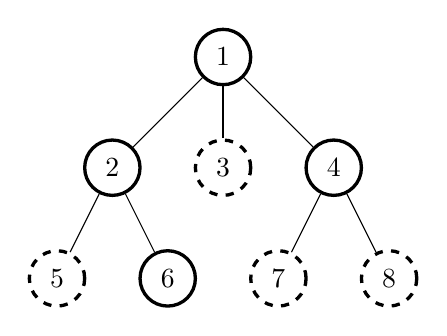
\begin{tikzpicture}[level distance=4em,sibling distance=4em,]
        
        \node (a1) [cir1] {1}
        child { node (a2)[cir1] {2}
            child { node (a5)[cir2] {5} } 
            child { node (a6)[cir1] {6} }
        }
        child { node (a3)[cir2] {3}}		
        child { node (a4)[cir1] {4}
            child { node [cir2] {7} } 
            child { node [cir2] {8} }
        };
        \end{tikzpicture}
        \caption{Sample graph with numbered node of two types}
        \label{fig:example-traversal1}
    \end{figure}

    One of the potential complete traversals for the graph from Figure \ref{fig:example-traversal1} starting from the node 1 is \{1, 2, 3, 4, 5, 6, 7, 8\} using breadth first strategy or \{1, 2, 5, 6, 3, 4, 7, 8\} for depth first strategy. On the other hand, a conditional traversal of non-dashed nodes staring from the node 1 results in \{1, 2, 4, 6\}, \{1, 4, 2, 6\} or \{1, 2, 6, 4\}. The first two traversals corresponding to the breadth first strategy and the third one to the depth first strategy. 

    I also use the graph traversal to execute generative operations on a parallel graph, which is a special case of \textit{graph rewriting}. For example DG traversal is employed for bootstrapping (i.e. creating in parallel) the CG as was previously motivated in Section \ref{sec:architecture}.

    \begin{definition}[Generative Traversal]\label{def:generative-traversal}
        Generative traversal $g(M,G)$ of a source graph $G$ via an operation matrix $M$ is an operation resulting in the creation of the target graph $H$ by contextually applying generative operations to bring the latter into existence. The operation matrix $M$ is a set of tuples $(ctx,o,p)$ that link the visited source node context $ctx$ (as features of the node, the edge and previously visited neighbour) to a certain operation $o$ that is executed on the target graph $H$ with parameters $p$.
    \end{definition}

    \tikzset{
        sqr1/.style={
            rectangle,
            draw=black, very thick,
            minimum height=0.5em,
            inner sep=0.5em,
            text centered,
            align=center,
            anchor=center
        }
    }
    
    \begin{figure}[!ht]
        \centering
        \begin{subfigure}[t]{0.28\textwidth}
            \centering
            \begin{tikzpicture}[scale=1]
            \node (a1) [cir1] { };
            \node (a11) [right =0.1em of a1] {= create};
            \node (a2) [cir2, below =2em of a1] { };
            \node (a21) [right =0.1em of a2] {= extend};
            \end{tikzpicture}
            \caption{The rule set}
            \label{fig:example-traversal00}
        \end{subfigure}
        \begin{subfigure}[t]{0.3\textwidth}
            \centering
            \begin{tikzpicture}[scale=1][level distance=4em,sibling distance=4em,]
            \node (a1) [sqr1] {a}
            child { node (a2)[sqr1] {b}
                child { node (a5)[sqr1] {d} } 
            }
            child { node (a3)[sqr1] {c}};
            \end{tikzpicture}
            \caption{The target}
            \label{fig:example-traversal21}
        \end{subfigure}
        \begin{subfigure}[t]{0.4\textwidth}
            \centering
            \begin{tikzpicture}[scale=1][level distance=4em,sibling distance=8em,]
            \node (a1) [sqr1] {a: \{1, 3\}}
            child { node (a2)[sqr1] {b: \{2, 5\}}
                child { node (a5)[sqr1] {d: \{6\}} } 
            }
            child { node (a3)[sqr1, right=1em of a2] {c: \{4, 7, 8\}}};
            \end{tikzpicture}
            \caption{The explained target}
            \label{fig:example-traversal22}
        \end{subfigure} 
        \caption{The generative traversal result for Figure \ref{fig:example-traversal1} using create and extend operations}
        \label{fig:example-traversal2}
    \end{figure}

    Next I provide an rough description of what happens when a generative traversal is executed and the exact algorithm will be described in detail in Section \ref{sec:creation-constituency-graph}. For example lets assume that only two types of operation are needed for our task at hand. The first is to create a new node on the target graph once a non-dashed node is visited on the source graph. And, second, is to pass the dashed nodes without doing anything. This is schematically represented in Figure \ref{fig:example-traversal00}. Lets now apply these operations on traversing the example graph using the breadth first strategy following the order provided above: 1, 2, 3, 4, 5, 6, 7, 8. The traversal graph is considered source graph and the target graph is empty at the beginning of the process. Upon visiting node 1 a first node is created on the target graph which is labelled \textit{a}. When traversing nodes 2 and 4 then each of them signal creation of the nodes \textit{b} and \textit{c} as children of \textit{a} in the target graph and correspondingly node 6 signals creation of node \textit{d}. The final target graph is depicted in Figure \ref{fig:example-traversal21} and in Figure \ref{fig:example-traversal22} the source nodes are embedded into the target node to make explicit that the non-dashed nodes (i.e. 3, 5, 7, 8) are simply passed over without any generative operation. 

    Now that generative traversal is defined, by analogy, \textit{update}, \textit{insert} and \textit{delete} traversals can be defined on the source or target graph by using the same mechanism of \textit{operation matrices} mapping contexts of visited nodes and edges to update, insert and delete operations. In this work, however, these operations are not used and could be explored in future work if needed.

    In Section \ref{sec:graphs} the last two definitions were for the constituency and dependency graphs. They are used in this thesis to represent grammatical analysis of a sentence. Next we will look at a special type of graph which represents fragments of structure repeatable across multiple analyses. They represent generalisations or patterns that usually are associated with grammatical features or a set of features which I explain in Chapter \ref{ch:parsing-algorithm}. These graphs are called \textit{pattern graphs} and the next section is dedicated to them.  

\section{Pattern graphs}
\label{sec:pattern-graphs}
    Regardless of the type, constituency or dependency, the parsing process (which will be described in Chapter \ref{ch:parsing-algorithm}) relies on identifying patterns in graphs. The patterning is described as both graph structure and feature presence (or absence) in the nodes or edges. The \textit{pattern graphs} (defined in \ref{def:graph-pattern}) are special kinds of graphs meant to represent small (repeatable) parts of parse graphs that, in the context of the current work, are used to identify grammatical features. 

    The pattern graphs contrast with the \textit{parse} (or \textit{instance}) graphs which are either constituency or dependency graphs. The parse graphs express what is an actual analysis of a text, i.e. representing what is the case, whereas the pattern graph expresses a potential that could be the case in the instance graph. This way the pattern graphs have a prescriptive interpretation whereas the instance ones take a factual interpretation. 

    %Pattern graphs can also specify operations that shall be executed when the pattern is successfully matched (for example add a new feature on a given node). This kinds of graphs need last four requirements listed in the beginning of this section.

    \begin{definition}[Pattern Graph]\label{def:graph-pattern}
        A \textit{pattern graph} (PG) is a feature rich graph for expressing regularities in the node and edge structure.
    \end{definition}

%part of the definition: or edge configuration and feature structure including descriptions of \textit{negated nodes or edges} (i.e. absence of), logical operators over feature sets (AND, OR, XOR and NAND) and operations once the pattern is identified in a target graph (select, insert, delete and update).

%The feature structure of a PG are always \textit{underspecified} as compared to the dependency or constituency graph in the sense that irrelevant attribute-value pairs are omitted sometimes down to an empty FS. However often it is useful to specify more than one value for the same feature as a list of disjunctive values allowing the pattern to cover larger set of possible cases. I will call these FS as being \textit{over-specified}. 

%An example of PG is depicted in figure \ref{fig:gp1} in the Section \ref{sec:pattern-graph-matching}. It deals with pattern graph matching and other operations with in detail. But before that I will first briefly cover generic operations on graphs and the problem of graph matching also known in computer science as the \textit{graph isomorphism} problem.

%Before I dive into characterising pattern graph matching and operations with pattern graphs, I 
    I discuss two example of pattern graphs. One example shows a pattern graph encoding the present perfect continuous tense, which traditional grammar defines as in Table \ref{tab:ppc-pattern}. Afterwards, the second example will show how the notion of linear succession among nodes is accounted for in the pattern graphs for declarative and interrogative mood.

    \begin{table}[!ht]
    	\centering
    	\begin{tabular}{|clclc|}
    		\hline
    		\textit{has/have}       & + & \textit{been}          & + & \textit{Vb-ing}          \\
    		to have, present simple &   & to be, past participle &   & verb, present participle \\ \hline
    	\end{tabular}
    	\caption{Present perfect continuous tense}
    	\label{tab:ppc-pattern}
    \end{table}

    Examples \ref{ex:ppc1}--\ref{ex:ppc3} show variations of present perfect continuous tense in a simple clause according to declarative and interrogative mood and ``has'' contraction. Of course there are more variations possible, for example, according to voice (active and passive), but they are omitted here because they add combinatorially to the number of examples and the ones provided already serve their purpose here. Figures \ref{fig:ppc1}-\ref{fig:ppc3} represent corresponding dependency parses for these examples (generated with the Stanford dependency parser).

    \begin{exe}
    	\ex\label{ex:ppc1} He has been reading a text.
    	\ex\label{ex:ppc2} He's been reading a text.
    	\ex\label{ex:ppc3} Has he been reading a text?
    \end{exe}

    %\begin{figure}[!ht]
    %	\centering
	\begin{figure}[!ht]
		\centering
		\begin{dependency}[dep-style-narrow]
			\begin{deptext}[]
				PRP \& VBZ \& VBN \& VBG \& DT \& NN \\
				He \& has \& been \& reading \& a \& text \\
			\end{deptext}
			\deproot{4}{root}
			\depedge{4}{1}{nsubj}
			\depedge{4}{2}{aux}
			\depedge{4}{3}{aux}
			\depedge{4}{6}{dobj}
			\depedge{6}{5}{det}
		\end{dependency}
		\caption{Present perfect continuous: indicative mood, un-contracted ``has''}
		\label{fig:ppc1}
	\end{figure}

	\begin{figure}[!ht]
        \centering
		\begin{dependency}[dep-style-narrow]
			\begin{deptext}[]
				PRP \& VBZ \& VBN \& VBG \& DT \& NN \\
				He \& 's \& been \& reading \& a \& text \\
			\end{deptext}
			\deproot{4}{root}
			\depedge{4}{1}{nsubj}
			\depedge{4}{2}{aux}
			\depedge{4}{3}{aux}
			\depedge{4}{6}{dobj}
			\depedge{6}{5}{det}
		\end{dependency}
		\caption{Present perfect continuous: indicative mood, contracted ``has'' }
		\label{fig:ppc2}
	\end{figure}
    %\end{figure}
    %
    \begin{figure}[!ht]
	\centering
	\begin{dependency}[dep-style]
		\begin{deptext}[]
			VBZ \& PRP \& VBN \& VBG \& DT \& NN \\
			Has \& he \& been \& reading \& a \& text \\
		\end{deptext}
		\deproot{4}{root}
		\depedge{4}{2}{nsubj}
		\depedge{4}{1}{aux}
		\depedge{4}{3}{aux}
		\depedge{4}{6}{dobj}
		\depedge{6}{5}{det}
		%\depedge[collage]{5}{6}{dobj}
	\end{dependency}
	\caption{Present perfect continuous: interrogative mood, un-contracted ``has''}
	\label{fig:ppc3}
    \end{figure}


    The present perfect continuous tense can be formulated as a pattern graph (including voice) over the dependency structure as illustrated in Figure \ref{fig:gp1}. In this pattern the main lexical verb is \textit{present participle} indicated via the \textit{VBG} part of speech. It is accompanied by two auxiliary verbs: \textit{to be} in \textit{past participle} (\textit{VBN}) form and \textit{to have} in \textit{present simple} form specified by either \textit{VBZ} for 3rd person or \textit{VBP} for non-3rd person. Also the \textit{to be} can be either connected by the \textit{aux} relation or in case of passive form by the \textit{auxpass} relation. Note that the pattern in Figure \ref{fig:gp1} constrains the edge type (using an OR-set) to the verb \textit{to be} which can be either \textit{aux} or \textit{auxpass} and the part of speech of the verb \textit{to have} which can be \textit{VBZ} or \textit{VBP}.

    \begin{figure}[!ht]
        \centering
        \begin{tikzpicture}[tree-style,level distance=5em,]
        \node[pattern-node, anchor=center] (vb1){pos:VBG}
        child {node[pattern-node] {lemma:be\\pos:VBN} edge from parent node[left] {$_{OR}$[aux,auxpass]} }
        child {node[pattern-node] {lemma:have\\pos:$_{OR}$[VBZ,VBP]} edge from parent node[right] {aux}};
        \end{tikzpicture}
        \caption{The graph pattern capturing features of the present perfect continuous tense}
        \label{fig:gp1}
    \end{figure}

    One of the fundamental features of language is its \textit{sequentiality} and \textit{directionality}. This aspect is not inherent in graphs. In the simplest form, they just describe connections between nodes and are agnostic to any meaning or interpretation. Next, I introduce the way I deal with linear order in the pattern graphs. 

    %To demonstrate how the order will specified in the graph patterns, 
    Lets consider the clause mood and encode the distinction between \textit{declarative} and \textit{Yes/No interrogative} moods. In SFG these features are described in terms of the relative order of clause elements. If the finite is before the subject then the mood is Yes/No-interrogative, whereas when the finite succeeds subject then the mood is declarative. Example \ref{ex:ppc3} contrasts in mood with Examples \ref{ex:ppc1} and \ref{ex:ppc2}. 

    Order can be specified in absolute or relative terms and partially or exhaustively. In order to cover these three kinds of constraints, I introduce three special features: the node \textit{id}, \textit{precede} and \textit{position}. Node id takes a token to uniquely identify a node in the graph, the precede feature takes an ordered set to indicate the (partial) linear precedence to other node ids, and the position feature indicates the absolute position of a node.

    One way to introduce order among nodes is then by marking them with an absolute position. This is a good method applicable to parse graphs. The DGs and CGs, are automatically assigned at creation time with the absolute position of the node in the sentence text via the feature \textit{position}. This feature is present in the leaf nodes only and corresponds to the order number in which they occur in the sentence text while the non-leaf node's position is considered to be the lowest position of its constituent nodes. The absolute position description is rarely used in the PGs. The only cases are to state that the constituent is in first or last position in a sentence.  %In the 

    Another way to specify node order is through relative precedence, for which the node id and the precedence features are introduced above. This is the preferred method to provide the linear precedence dimension in pattern graphs. It is also relative so the specification can be partial. With this method a node specifies that it precedes a set of other nodes. 

	\begin{figure}[!ht]%{0.4\textwidth}
		\centering
		\begin{tikzpicture}[tree-style,,level distance=4em,]
		\node (cla) [pattern-node] {class:clause}
		child { node (sub)[pattern-node] {element:subject,\\position:1}}		
		child { node (f)[pattern-node] {element:finite,\\position:2}};
		\end{tikzpicture}
		\caption{Declarative mood pattern graph with absolute element order}
		\label{fig:pg-declarative}
	\end{figure}
	\begin{figure}[!ht]%{0.4\textwidth}
		\centering
		\begin{tikzpicture}[tree-style,,level distance=4em,]
		\node (cla) [pattern-node] {class:clause}
		child { node (sub)[pattern-node] {element:subject,\\id:s1, precede:f1}}		
		child { node (f)[pattern-node] {element:finite,\\id:f1}};
		\end{tikzpicture}
		\caption{Declarative mood pattern graph with relative element order}
		\label{fig:pg-declarative2}
	\end{figure}
    \begin{figure}[!ht]
    	\centering
    	\begin{tikzpicture}[tree-style,,level distance=4em,]
    	\node (cla) [pattern-node] {class:clause}
    	child { node (f)[pattern-node] {element:finite,\\id:f1, precede:s1}}
    	child { node (sub)[pattern-node] {element:subject,\\id:s1}}	;	
    %	child { node (mv)[pattern-node] {element:main verb,\\id:mv1}};
    	\end{tikzpicture}
    	\caption{Pattern graph for Yes/No interrogative mood}
    	\label{fig:pg-interrogative}
    \end{figure}

    To continue the example of mood features, I illustrate in Figures \ref{fig:pg-declarative} and \ref{fig:pg-declarative2} the use of relative and absolute node ordering constraints for declarative mood; and in Figure \ref{fig:pg-interrogative}, I depict the PG for the Yes/No interrogative mood. In both the latter cases I use relative node ordering.

    %todo: explain what negative nodes are
    
    %From the usability point of view there are few technicalities I shall emphasize. First, the precedence feature can be used on any node. When matched, the precedence declarations are collected from all nodes into a single set before being checked. However I recommend as a good practice to specify the order of nodes on the parent constituent. 
    %
    %Second, the notation in Figure \ref{fig:pg-interrogative} follows the Python bracketing meaning i.e. the round brakes signify tuples while the square ones lists (ordered sets). So the main verb element is redundant and is introduced to demonstrate multiple order specifications. However the order can be either specified as a set of binary tuples or as an ordered set (i.e. a Python list). So precedence:[(f1,s1),(s1,mv1)] is equivalent to precedence:[f1,s1,mv1]. 
    %
    %Thirdly the ordering can be defined in absolute terms via position or in relative terms. Note that in the case of PGs the absolute ordering of nodes is interpreted relatively so PG in figure \ref{fig:pg-declarative} is identical to \ref{fig:pg-declarative2}.

    Patterns like the ones explained above can be created for a wide range of grammatical features. Once the grammatical feature is encoded as a pattern graph it can be identified in parse graphs (DG or CG) via the \textit{graph pattern matching} operation described in Section \ref{sec:graph-matching}. Moreover, once the pattern is identified it can act as a triggering condition for the node update operation. When the pattern is matched then additional features can be added to the nodes of the parse graph and is the mechanism of enriching the parse graph. Coming back to out tense example above, once the pattern \ref{fig:gp1} is identified then the clause can be marked with the tense feature. In the next section I address the graph matching operation and then show how it works using pattern graphs. 

    % skip:complicated, unclear, compressed
    %But such traversal operations cannot be easily defined. While traversal context may be sufficient for generative operations on a new structure, it is insufficient for executing affecting operations on the traversed graph. To overcome this limitation, instead of using traversal context I take a different approach: the \textit{pattern graphs}, defined in previous section combined with generic graph matching algorithm. This mechanism offers a similar algorithmic independence of mapping structural context to operation(s) triggered by it. 

\section{Graph matching}
\label{sec:graph-matching}

    So far we have discussed about constituency and dependency graphs and, in the last section, I introduced pattern graphs. The intuition behind pattern graphs is that they are meant to be matched against or found in other graphs. The patterns graphs can be viewed as small reusable modules and as generalisations consisting of structural patterns. I will address next what it means for two graphs to be the same, i.e. \textit{isomorphic} and how this sameness checking is used in the current work. 

    In \textit{mathematics} structure-preserving mappings $f:X \rightarrow Y$ (from one object $X$ to the other $Y$) of the same type are called \textit{morphisms}. The morphism $f:X \rightarrow Y$ is called an \textit{isomorphism} if there exists an inverse morphism $g:Y \rightarrow X$ such that $f \circ g = id_{X}$ and $ g \circ f = id_{X}$.

    %\begin{definition}[Morphism]\label{def:morphism}
    %    A morphism $f:X \rightarrow Y$ is a structure preserving map from one object $X$ to the other $Y$ where the objects are complex structures such as sets, feature structures or graphs.
    %\end{definition}
    %
    %
    %\begin{definition}[Isomorphism]\label{def:isomorphism}
    %    The morphism $f:X \rightarrow Y$ is called \textit{isomorphism} if there exists an inverse morphism $g:Y \rightarrow X$ such that $f \circ g = id_{X}$ and $ g \circ f = id_{X}$.
    %\end{definition}

    In computer science, the \textit{graph matching} operation is known as a (sub-)graph isomorphism. Two graphs $G=(V_G,E_G)$ and $H=(V_H,E_H)$ are isomorphic if there exists a mapping from the nodes of graph $G$ to the nodes of graph $H$, such that the edge neighbourhood is preserved. In such a context the nodes are unique atomic symbols functioning as node identifiers. 
 
    \begin{definition}[Graph matching]\label{def:gmatching}
        For two graphs $G$ and $H$, where $G \leq H$, \textit{graph matching} is the operation of finding an isomorphism between $G$ and $H$.
    \end{definition}

    \begin{definition}[Graph isomorphism]\label{def:gisomorphism}
        An isomorphism of graph $G=(V_G,E_G)$ and $H=(V_H,E_H)$ is a bijective function $f:V_G \rightarrow V_H$ such that if any two nodes  $u,v \in V_G$ from $G$ are adjacent $(u,v) \in E_G$ then $f(u), f(v)$ are adjacent in $H$ as well $(f(u), f(v)) \in E_H $.
    \end{definition}

    Graphs do not always have the same number of nodes (or edges). We say that a graph is smaller than another one, denoted $G \leq H$, when its number of nodes is less than that of the other graph. In such cases, for two graphs $G$ and $H$ where $G<H$, the (sub-)graph matching task is redefined to establishing isomorphism(s) from $G$ to a sub-graph of $H$. 
    %In this case, the mapping function is relaxed from bijective (perfect mapping from first to second graph) to an injective one (each node from first has a correspondent in the second one).

    \begin{definition}[Sub-graph isomorphism]\label{def:sgisomorphism}
           Given two feature rich graphs $G=(V_G,E_G)$ and $H=(V_H,E_H)$, $G$ is sub-graph isomorphic to $G$ (denoted $G \subseteq H$) if there is an injective function $f:V_G \rightarrow V_H$ such that
       \begin{itemize}
           \item $\forall v \in V_G, f(v) \in V_H$ and
           \item any two nodes adjacent in $G$, $(u,v) \in E_G$, are also adjacent in $H$, $(f(u), f(v)) \in E_H $
       \end{itemize}
    \end{definition}


    \begin{figure}[!ht]
        \centering
        \begin{subfigure}[t]{0.48\textwidth}
            \centering
            \begin{tikzpicture}[scale=1]
            \node (a1) [cir1] {1};
            \node (a2) [cir1, right =3em of a1] {2};
            \node (a3) [cir1, below =3em of a1] {3};
            
             \draw[sequence,->] (a1) -- (a2);
             \draw[sequence,->] (a2) -- (a3);
             \draw[sequence,->] (a3) -- (a1);
            
            \end{tikzpicture}
            \caption{The pattern graph}
            \label{fig:example-matching1}
        \end{subfigure}
        \begin{subfigure}[t]{0.48\textwidth}
            \centering
            \begin{tikzpicture}[scale=1][level distance=4em, sibling distance=4em,]
            \node (a1) [cir1] {a};
            \node (a2) [cir1, right =3em of a1] {b};
            \node (a3) [cir1, below =3em of a1] {c};
            \node (a4) [cir1, below =3em of a2] {d};
            
            \draw[sequence,->] (a1) -- (a2);
            \draw[sequence,->] (a2) -- (a3);
            \draw[sequence,->] (a3) -- (a1);
            \draw[sequence,->] (a2) -- (a4);
            
            \end{tikzpicture}
            \caption{The target graph}
            \label{fig:example-matching2}
        \end{subfigure}
        \caption{Sub-graph isomorphism \{1=a, 2=b, 3=c\}}
        \label{fig:example-matching}
    \end{figure}

    Figure \ref{fig:example-matching1} depicts a labelled graph that is isomorphic to a sub-graph in Figure \ref{fig:example-matching2}. The example graphs presented in Figure \ref{fig:example-matching} have atomic labels as nodes and the isomorphism is established as a mapping between labels. Section \ref{sec:graphs} above mentioned that the graphs considered in this thesis have feature structures as their nodes and no atomic nodes. But in case of feature rich graphs additional rules to establish the isomorphism need to be provided because there are multiple ways of approaching it. 

    \begin{figure}[!ht]
        \centering
        \begin{subfigure}[t]{0.38\textwidth}
            \centering
            \begin{tikzpicture}[scale=1]
            \node (a1) [pattern-node] {f_1: 1 \\ f_2: scissors};
            \node (a2) [pattern-node, right =3em of a1] {f_1: 2 \\ f_2: paper};
            \node (a3) [pattern-node, below =3em of a1] {f_1: 3 \\ f_2: rock};
            
            \draw[sequence,->] (a1) -- (a2);
            \draw[sequence,->] (a2) -- (a3);
            \draw[sequence,->] (a3) -- (a1);
            
            \end{tikzpicture}
            \caption{The pattern graph}
            \label{fig:example-r-matching1}
        \end{subfigure}
        \begin{subfigure}[t]{0.58\textwidth}
            \centering
            \begin{tikzpicture}[scale=1][level distance=4em, sibling distance=4em,]
            \node (a1) [pattern-node] {f_1: a \\ f_2: scissors};
            \node (a2) [pattern-node, right =3em of a1] {f_1: b \\ f_2: paper};
            \node (a3) [pattern-node, below =3em of a1] {f_1: c \\ f_2: rock};
            \node (a4) [pattern-node, below =3em of a2] {f_1: d \\ f_2: scissors};
            \node (a5) [pattern-node, right =3em of a4] {f_1: e \\ f_2: rock};
            
            \draw[sequence,->] (a1) -- (a2);
            \draw[sequence,->] (a2) -- (a3);
            \draw[sequence,->] (a3) -- (a1);
    
            \draw[sequence,->] (a2) -- (a4);
            \draw[sequence,->] (a4) -- (a5);
            \draw[sequence,->] (a5) -- (a2);
            
            \end{tikzpicture}
            \caption{The target graph}
            \label{fig:example-r-matching2}
        \end{subfigure}
        \caption{An example of rich sub-graph isomorphism}
        \label{fig:example-r-matching}
    \end{figure}

    Lets look at Figure \ref{fig:example-r-matching} where the graph nodes are feature structures using features: $f_1$ and $f_2$. One way to approach isomorphism in this scenario is by the value of one feature, for example $f_1$. Then we can identify two sub-graph isomorphisms: \{1=a, 2=b, 3=c\} and \{1=b, 2=d, 3=e\}. This approach, besides additional specification what values to compare, i.e. $f_1s$, is the same as providing a sub-graph isomorphism on the labelled graphs from Figure \ref{fig:example-matching}. 

    In addition to the rule above, lets add a constraint that the isomorphism is not only a mapping between the feature values (numbers to letters) but also that the mapped values are identical (strict value equality). If we consider the strict equality rule applied on $f_1$ feature, there is no isomorphism between the two graphs because first one uses numbers  \{1, 2, 3\} and the second uses letters\{a, b, c, d\}. Now if we turn to the values of $f_2$ and apply the same rule then there is one isomorphism possible \{paper=paper, rock=rock, scissors=scissors\}. The second one, even if it is a cycle, \{paper=paper, rock=scissors, scissors=rock\} is no longer acceptable because the ``scissors'' and ``rock'' switched places in the target graph; it would have been acceptable as a mapping, but not as strict value equality. Formally, the additional equality constraint can be expressed on the graph isomorphism $f$ as $u=f(u)$.

    This brings us to the idea that, in the feature rich (sub-)graph isomorphism, we need to introduce a \textit{matching} operator (denoted $\match$) for nodes. This means that we no longer can use atomic symbol mapping but have to employ the matching operator. The node matching operation is defined on feature structures. We say that a feature structure may match another feature structure once, several times or not at all, $FS_1 \match FS_2$. This intuition is expressed in Definition \ref{def:fs-match}. The sub-graph isomorphism over the feature rich graphs is captured in Definition \ref{def:rsgisomorphism} below.

    %For graph matching definition this implies that the node label equality operation is replaced with matching criteria is the method to impose an additional set of constraints on the graph isomorphism and allow comparison of complex nodes such as those in feature rich graphs. 
     
    %The rich graph matching operation can be also seen as a search for rich sub-graph isomorphism. 

    \begin{definition}[Rich sub-graph isomorphism]\label{def:rsgisomorphism}
        Given two feature rich graphs $G=(V_G,E_G)$ and $H=(V_H,E_H)$ and a matching relation $\match$, $G$ is a sub-graph isomorphic to $H$ if there is an injective mapping $f:V_G \rightarrow V_H$ such that
        \begin{itemize}
            \item each node in $V$ is mapped to exactly one node in $H$, $\forall v \in V_G, f(v) \in V_H$ and
            \item each node in $G$ matches with its correspondent in $H$, $\forall v \in V_G, v \gtrdot f(v)$ and
            \item any two nodes which are adjacent in $G$, are also adjacent in $H$, $\forall (u,v) \in E_G, \exists \big(f(u), f(v)\big) \in E_H $
        \end{itemize}
    \end{definition}

    %\begin{definition}[Rich Graph Matching]\label{def:rgmatching}
    %    For two feature rich graphs $G$ and $H$ where $H \leq G$ and an \textit{identity settling function} $idx_{V}$, the \textit{rich graph matching} is the function that finds a structural isomorphism between $H$ and $G_{1} \subseteq G$ provided that for all nodes $V_{i} \in H$ their \textit{morphism function} $V_{j} \in G_{1}$ 
    %    
    %    satisfies the identity function $f_{V}(V_{i})=V_{j}$ 
    %\end{definition}
    
    %The congruency rules (also referred in the implementation as \textit{identity} or \textit{equivalence functions}) used in this work will be provided in the Section \ref{sec:pattern-graph-matching} below. They are contextualised to the graph matching operation between pattern graphs and dependency and constituency graphs. 
    %
    %\section{Pattern graph matching}
    %\label{sec:pattern-graph-matching}

    We already mentioned in the introduction of this section that pattern graphs are considered as generalisations over parse graphs (constituency or dependency). The pattern graphs are smaller and their nodes have fewer features specified. The parse graphs have more nodes and features. We say that a parse graph \textit{instantiates} a pattern graph if there exists a rich sub-graph isomorphism. This operation is called \textit{pattern graph matching} and is defined in Definition \ref{def:pgmatching} below. 

    \begin{definition}[Pattern graph matching]\label{def:pgmatching}
        Given a pattern graph $G$ and an instance (parse) graph $H$ (either dependency or constituency), \textit{pattern graph matching} is the operation of finding a rich sub-graph isomorphism from $G$ to $H$ such that each pattern node matches its corresponding instance node for each $H$, $\forall v \in V_G, v \gtrdot f(v)$.
    \end{definition}

%The pattern and parse graphs are feature rich graphs. This means that the nodes are feature structures. In the previous section the rich graph matching require definition of congruence rules and in this case it is between two feature structures. 

    As mentioned before, nodes of the parse and the pattern graphs are feature structures. I approach the matching between them in two steps: first, matching the feature names in Definition \ref{def:fs-match}, and second,  matching the feature values in Table \ref{tab:strict}. In order to simplify and make explanations clear, I will further refer to the feature structures that constitute nodes in the pattern graphs as \textit{pattern feature structures} and the feature structures that constitute nodes in the instance graphs as \textit{instance feature structures}.

    \begin{definition}[Feature structure matching]\label{def:fs-match}
        A pattern feature structure $V$ matches an instance feature structure $U$ if and only if every feature in $V$ has a corresponding feature $U$ and their values match; that is $ \forall f_V \in V, \exists f_U$ such that $name(f_V) = name(f_U)$ and $ val(f_V) \match val(f_U)$.
    \end{definition}

    %Next is defined matching of the feature values. 
    According to Definition \ref{def:fs}, the values of feature structures can be either atomic (numbers, strings, symbols, etc.), denoted $atomic$, or one of the conjunction sets: $S_{AND}$, $S_{OR}$, $S_{XOR}$ and $S_{NAND}$. For simplicity, the option of nested feature structures is excluded in the current work even though it is perfectly viable configuration. Consequently, the matching relation takes into consideration the \textit{type} of the compared elements in addition to how they relate to each other, including comparisons between set and atomic values. Note that this relation is \textit{not symmetric}, i.e. \textit{not commutative} because the subsequent relations used in the definition, i.e. set inclusion and set subsumption, are not symmetric. This means that $A \match B \neq B \match A $. 
    %Finally, these definitions create equivalence sets \textit{relative} to one of the compared elements and not absolute equivalence sets. For example the division by 2, is an absolute condition for two numeric elements to belong to the same equivalence class either of odd or that of even numbers. By contrast, if we consider set inclusion between two sets $A \subseteq B$ as a condition for set element equivalence then it generates two possible equivalence sets. First, all sets $X$ that are subsets of $B$, $\forall X, X \subseteq B$ and second, all sets Y that include $A$,  $ \forall Y, A \subseteq Y $. 

    I will also remind here that the function $\tau(S)$, defined in Section \ref{sec:graphs}, returns the \textit{type} of the feature value. I extend its definition here to handle also atomic data types as follows: $\tau:x \rightarrow \{atomic, S_{AND}, S_{OR}, S_{XOR}, S_{NAND} \}$. The matching rules have to be defined for each possible pair of types returned by the function $\tau$ yielding 25 possibilities. Table \ref{tab:strict} provides matching relations for each pair of types where the rows represent value types of the pattern features, denoted $\tau(v)$, and the columns represent value types of the instance features, denoted $\tau(u)$. Each table cell contains a comparison expression returning a truth value. Cells with a bottom sign $\bot$ mean that there can be no match between these types no matter the values. 
    %I use set theoretic notations such as set inclusion $\subseteq$, intersection $\cup$ and set membership $\in$. 

    \begin{table}[!ht]
        \centering
        \begin{tabular}{|c|c|c|c|c|c|}
            \hline
            \textit{$\tau(v)$\textbackslash $\tau(u)$} & \textit{atomic} & \textit{S_{AND}}                 & \textit{S_{OR}}              & \textit{S_{XOR}}             & \textit{S_{NAND}}            \\ \hline
            \textit{atomic}             & $v=u$             & $v \in u$                         & $\bot$                          & $\bot$                          & $v \notin u$                   \\ \hline
            \textit{S_{AND}}              & $\bot$               & $v \subseteq u$                     & $\bot$                          & $\bot$                          & $\bot$ \\ \hline
            \textit{S_{OR}}               & $v \ni u$          & $ v \cap u \neq \varnothing $ &                        $v \supseteq u $              & $v \supseteq u $   & $\bot$ \\ \hline
            \textit{S_{XOR}}              & $v \ni u$          & $\bot$                              & $\bot$                        & $v \supseteq u$             & $\bot$ \\ \hline
            \textit{S_{NAND}}             & $v \not\ni u$      & $v \cap u = \varnothing$     & $v \cap u = \varnothing$ & $v \cap u = \varnothing$ & $ v \subseteq u $                          \\ \hline
        \end{tabular}
        \caption{Strict matching between pattern and instance feature values organised by value type}
        \label{tab:strict}
    \end{table}

    For example, if both values are of atomic type then in order to match they have to equal. If the $\tau(v)$ is atomic and the $\tau(u)$ is an AND set then $v$ needs to be among the set of values constituting $u$; whereas if the $\tau(u)$ is an OR or XOR set then these values do not match, designated by the bottom sign $\bot$. The same reading applies to the rest of the table for each pair of value types. 

    A more permissive matching is defined in Table \ref{tab:permissive}. Here, on the instance feature values, the two types of disjunction (OR and XOR) and the negated conjunction (NAND) are interpreted as possibly matching and are provided with the corresponding relation, whereas in the previous definition these cases were completely excluded. The permissive match is rarely used in this work but it is nevertheless useful for cases of instance graphs where the feature values could not be assigned with a certainty but as a disjunction of either one or the other. 

    \begin{table}[!ht]
        \centering
        \begin{tabular}{|c|c|c|c|c|c|}
            \hline
            \textit{$\tau(v)$\textbackslash $\tau(u)$} & \textit{atomic} & \textit{S_{AND}}                 & \textit{S_{OR}}              & \textit{S_{XOR}}             & \textit{S_{NAND}}            \\ \hline
            \textit{atomic}             & $v=u$             & $v \in u$                         & $v \in u$                          & $v \in u$                          & $v \notin u$                   \\ \hline
            \textit{S_{AND}}              & $\bot$               & $v \subseteq u$                     & $v \subseteq u$                          & $v \subseteq u$                          & $v \cap u = \varnothing$ \\ \hline
            \textit{S_{OR}}               & $v \ni u$          & $ v \cap u \neq \varnothing $ &                        $v \supseteq u $              & $v \supseteq u $   & $v \backslash u \neq \varnothing$ \\ \hline
            \textit{S_{XOR}}              & $v \ni u$          & $\bot$                              & $\bot$                        & $v \supseteq u$             & $ |v \backslash u| = 1$ \\ \hline
            \textit{S_{NAND}}             & $v \not\ni u$      & $v \cap u = \varnothing$     & $v \cap u = \varnothing$ & $v \cap u = \varnothing$ & $ v \subseteq u $                          \\ \hline
        \end{tabular}
        \caption{Permissive matching between pattern and instance feature values organised by value type}
        \label{tab:permissive}
    \end{table}


    %the old taxt no longer needed
    %
    %
    %When checking the equivalence of two feature values, three cases can be asserted: $x=y$ i.e. $x$ is definitely equal to $y$, $x\neq y$ i.e. $x$ is definitely different from $y$ and $x\sim y$ i.e. $x$ is maybe (or could be) equal to $y$. 
    %
    %I define below two identity morphisms: (a) \textit{permissive} $I_{permissive}$ (defined by Equation \ref{eq:permissive}) which includes the uncertain cases and (b) \textit{strict} $I_{strict}$ (defined by Equation \ref{eq:strict}) which excludes the uncertain cases. The main difference between the two morphism functions is whether on the right side (the instance graph) any uncertainty is accepted. This is to say any of the disjunctive sets $s_{OR}$ and $S_{XOR}$. 
    %
    %\begin{definition}[Strict Pattern Graph Matching]\label{def:strict-matching}
    %	\textit{Strict pattern graph matching} is a rich graph matching where a morphism for the pattern graph $H$ is found in the target graph $G$ given that $H \leq G$ and that for any node $p \in H$ there is a node $r \in G$ satisfying the strict identity morphism $I_{strict}:p \rightarrow r$
    %\end{definition}
    %
    %
    %\begin{equation} \label{eq:strict}
    %	I_{strict}:p \rightarrow r \models
    %	\begin{cases}
    %	p = r, & \text{if}\ T(p) = simple \wedge T(r) = simple \\
    %	p \in r, & \text{if}\ T(p) = simple \wedge T(r) = S_{AND} \\
    %	p \subseteq r, & \text{if}\ T(p) = S_{AND} \wedge T(r)= S_{AND} \\
    %	p \cap r \neq \varnothing, & \text{if}\ T(p) = S_{OR} \wedge T(r) = S_{AND}\\
    %	r \in p, & \text{if}\ T(p) = S_{OR} \wedge T(r) = simple \\
    %	%p \cap r \neq \varnothing, & \text{if}\ T(p) = S_{XOR} \wedge T(r) \in \{S_{OR}, S_{XOR}\} \\
    %	r \in p, & \text{if}\ T(p) = S_{XOR} \wedge T(r) = simple \\
    %	p \cap r = \varnothing, & \text{if}\ T(p) = S_{NAND} \wedge T(r) \in \{S_{AND}, S_{OR}, S_{XOR}\} \\
    %	r \notin p, & \text{if}\ T(p) = S_{NAND} \wedge T(r) = simple \\
    %	\top, & \text{if}\ T(p) = S_{NAND} \wedge T(r) = S_{NAND}
    %	\end{cases}
    %\end{equation}
    %
    %\begin{definition}[Permissive Pattern Graph Matching]\label{def:permissive-matching}
    %	\textit{Permissive pattern graph matching} is a rich graph matching where a morphism for the pattern graph $H$ is found in the target graph $G$ given that $H \leq G$ and that for any node $p \in H$ there is a node $r \in G$ satisfying the permissive identity morphism $I_{permissive}:p \rightarrow r$
    %\end{definition}
    %
    %\begin{equation} \label{eq:permissive}
    %	I_{permissive}:p \rightarrow r \models
    %	\begin{cases}
    %	p = r, & \text{if}\ T(p) = simple \wedge T(r) = simple \\
    %	p \in r, & \text{if}\ T(p) = simple \wedge T(r) \in \{S_{AND}, S_{OR}, S_{XOR}\} \\
    %	p \subseteq r, & \text{if}\ T(p) = S_{AND} \wedge T(r) = S_{AND} \\
    %	p \cap r \neq \varnothing, & \text{if}\ T(p) = S_{OR} \wedge T(r) \in \{S_{AND}, S_{OR}, S_{XOR}\}\\
    %	r \in p, & \text{if}\ T(p) = S_{OR} \wedge T(r) = simple \\
    %	p \cap r \neq \varnothing, & \text{if}\ T(p) = S_{XOR} \wedge T(r) \in \{S_{OR}, S_{XOR}\} \\
    %	r \in p, & \text{if}\ T(p) = S_{XOR} \wedge T(r) = simple \\
    %	p \cap r = \varnothing, & \text{if}\ T(p) = S_{NAND} \wedge T(r) \in \{S_{AND}, S_{OR}, S_{XOR}\} \\
    %	r \notin p, & \text{if}\ T(p) = S_{NAND} \wedge T(r) = simple \\
    %	\top, & \text{if}\ T(p) = S_{NAND} \wedge T(r) = S_{NAND}
    %	\end{cases}
    %\end{equation}
    
    %The matching rules proposed in Definition \ref{def:fs-match} and Table \ref{tab:strict} are not the only one that can be defined for the pattern matching. 
    %A more permissive forms are possible, for example checking subset set inclusion for OR and XOR sets which currently is excluded.   
    %To handle this possible variation, in the parser implementation, the pattern matching function takes as parameter the FS matching function. The only constraints are to return a truth value and to take two parameters. The implementation also supports identity function for edges as well. In this work, all the pattern matching is performed entirely on constituent graphs (whose edges have no labels) and none on the dependency graphs (whose edges have labels), therefore I skip entirely the discussion about the edge matching in a sub-graph isomorphism. Nonetheless, the matching definitions above apply to matching edge features feature values too. 

    The permissive FS matching has been developed together with the strict FS matching as it was not clear at the beginning of the work which one is suitable for current purposes. After conducting several tests it became clear that strict matching is the one yielding the better results because it yields fewer matches. This is especially visible in the cases of Transitivity enrichment when too many incorrect patterns are qualified by the permissive operator. Now that pattern graph matching is explained, lets take a look next at how it is used to perform operations on instance graphs.

\section{Pattern based operations}
\label{sec:pattern-based-operations}

    Patterns are searched for in a graph always for a purpose. Graph isomorphism is only a precondition for another operation, be it a simple selection (i.e. non-affecting operation) or an affecting operation such as feature structure enrichment (on either nodes or edges), inserting or deleting a node or drawing a new connection between nodes. It seems only natural that the end goal is embedded into the pattern, so that when it is identified, also the desired operation(s) is(are) triggered. I call such graph patterns \textit{operational pattern graphs} (Definition \ref{def:operational-pattern}). Next I explain how to embed  operations into the graph pattern and how they are used in the parsing algorithm. 

        \begin{definition}[Operational graph pattern]\label{def:operational-pattern}
            An \textit{operational graph pattern} is a pattern graph that has at least on one node \textit{operation} and \textit{arg} features.
        \end{definition}

    The operational aspect of the pattern graph is specified in the node FS via three special features: \textit{id}, \textit{operation} and \textit{arg}. The \textit{id} feature (the same as for relative node ordering) is used to mark the node for further referencing as an argument of an operation, the \textit{operation} feature names the function to be executed once the pattern is identified and the \textit{arg} feature specifies the function arguments if any are required; they are tightly coupled with function implementation. If a node has the feature operation then it is called an \textit{operational node}. Also, in the current implementation, the special features such as operation, arg, id, precede etc. are excluded from the pattern matching operation because they have functional roles linked to the implementation and do not describe the linguistic properties of a graph node.

    So far the implemented operations are \textit{insert}, which is used for creation of empty nodes, \textit{delete}, which is used for corrections of predictable errors in dependency graphs and the \textit{update} operation, which is the main mechanism behind graph enrichment. These operations are depicted in Figure \ref{fig:pipeline-overview} of the parser pipeline architecture from Section \ref{sec:architecture}.

    Operative patterns are enacted once they are matched to an instance graph. An operative pattern graph $G$ is \textit{enacted} on an instance graph $H$, in two steps. First, the pattern graph is strictly matched to an instance graph. If an isomorphism $f$ is found then, second, for every operational node $v \in G, \exists att(v)=operation$, the specified operation $op = val(v.operation)$ and the corresponding node of the instance graph $u \in H$, the operation is executed on the node of the instance graph $op(u)$. If the arg feature is provided then the operation is executed with that additional argument. 

\subsection{Pattern based node update} 

    As mentioned above the pattern based node update is used for adding onto the constituency graph new features. Lets consider Example \ref{ex:transitivity1} whose constituency graph is provided in Figure \ref{fig:cg-transitive1} and the task is to assign the \textit{agent} feature to the subject node and \textit{affected-possessed} feature to the complement. This can be done using the pattern graph matching with a feature update operation indicated on subject and complement nodes. The PG depicted in Figure \ref{fig:pg-transitive1} fulfils this purpose because it matches the constituency graph from Figure \ref{fig:cg-transitive1} and has the corresponding update operations indicated.

    \begin{exe}
        \ex\label{ex:transitivity1} He gave the cake away.
        \ex\label{ex:transitivity2} He gave her the cake.
    \end{exe}

    %\begin{table}[!ht]
    %    \centering
    %    \begin{tabular}{|c|c|c|c|c|}
    %        \hline
    %        \multicolumn{5}{|c|}{clause}                                                               \\ \hline
    %        subject & main verb & \multicolumn{2}{c|}{complement} & adjunct \\ \hline
    %        He              & gave               & the               & cake               & away.            \\ \hline
    %    \end{tabular}
    %    \caption{CG with a transitive verb}
    %    \label{tab:transitive1}
    %\end{table}
    
    %The constituency graph representation for the clause analysis from Table \ref{tab:transitive1} is depicted in Figure \ref{fig:cg-transitive1}. 

    \begin{figure}[!ht]
        \centering
        \scalebox{0.7}{
        \begin{tikzpicture}[
        tree-style, 
    %    edge-style,
        level 1/.style={sibling distance=10em},
        level 2/.style={sibling distance=8em},
        level distance = 4em
        ]
        \node[pattern-node]{class: clause}
        child {node[pattern-node]{element: subject\\word: He} }
        child {node[pattern-node]{element: main verb\\word: gave} }
        child {node[pattern-node]{element: complement\\class: nominal group}  {}
            child {node[pattern-node]{element: deictic\\word: the} }
            child {node[pattern-node]{element: thing\\word: cake} }
        }
        child {node[pattern-node]{element: adjunct\\word: away}  }
        ;
        \end{tikzpicture}
    }
        \caption{Constituency graph corresponding to Example \ref{ex:transitivity1}}
        \label{fig:cg-transitive1}
    \end{figure}
    \begin{figure}[!ht]
    \centering
    \scalebox{0.7}{
    \begin{tikzpicture}[tree-style, level 1/.style={sibling distance=14em}, level distance = 5em]
    \node[pattern-node]{element:clause}
    	child {node[pattern-node, xshift=1.5em]{element: subject\\operation: update\\arg1:\{participant: agent\}} }
       	child {node[pattern-node]{element: main verb\\word: give\\operation: update\\arg1:\{process: possessive\}} }
        child {node[pattern-node, xshift=1em]{element: complement\\operation: update\\arg1:\{participant: affected-possessed\}}};
    \end{tikzpicture}
    }
    \caption{A graph pattern for inserting agent and affected-possessed participant roles}
    \label{fig:pg-transitive1}
    \end{figure}
    \begin{figure}[!ht]
        \centering
        \scalebox{0.7}{
            \begin{tikzpicture}[
            tree-style, 
            %    edge-style,
            level 1/.style={sibling distance=12em},
            level 2/.style={sibling distance=8em},
            level distance = 5em
            ]
            \node[pattern-node]{class: clause}
            child {node[pattern-node, xshift=2em]{element: subject\\\textit{participant: agent}\\word: He} }
            child {node[pattern-node]{element: main verb\\\textit{process: possessive}\\word: gave} }
            child {node[pattern-node]{element: complement\\\textit{participant: affected-possessed}\\class: nominal group}  {}
                child {node[pattern-node]{element: deictic\\word: the} }
                child {node[pattern-node]{element: thing\\word: cake} }
            }
            child {node[pattern-node]{element: adjunct\\word: away}  }
            ;
            \end{tikzpicture}
        }
        \caption{The resulting constituency graph enriched with participant roles}
        \label{fig:cgg-transitive1}
    \end{figure}

    Consider the same pattern, but applied to a sentence in Table \ref{tab:di-transitive1}. This clause has two complements and they are by no means distinguished in the pattern graph. When such cases are encountered the PG yields two matches (each with another complement) and the update operation is executed on both of the complements. To overcome such cases the  PG allow defining \textit{negative nodes}, meaning that those are nodes that shall be missing in the target graph.

    For example to solve the previous case I define the PG depicted in Figure \ref{fig:gp4} whose second complement is a negative node and it is marked with dashed line. This pattern is matched only against clauses with exactly one complement leaving aside the di-transitive ones because of the second complement.

    \begin{table}[!ht]
    \centering
    \begin{tabular}{|c|c|c|c|c|}
    \hline
    \multicolumn{5}{|c|}{class:clause}                                                                  \\ \hline
    element:subject & element: main verb & element:complement & \multicolumn{2}{c|}{element:complement} \\ \hline
    He              & gave               & her                & the               & cake.               \\ \hline
    \end{tabular}
    \caption{CG with a di-transitive verb}
    \label{tab:di-transitive1}
    \end{table}
    
    \begin{figure}[hbtp]
    \centering
    \scalebox{0.8}{
    \begin{tikzpicture}[tree-style,level distance=5em, level 1/.style={sibling distance=12.5em},]
    \node[pattern-node, anchor=center](vb1){element:clause}
    	child {node[pattern-node,xshift=0em] {element:subject,\\operation:update,\\ arg1:\{participant:agent\}} edge from parent node[above] {}}
    	child {node[pattern-node,xshift=0em] {element:complement,\\operation:update,\\ arg1:\{participant:posessed\}} edge from parent node[below right] {}}
    	child {node[pattern-node-negative, xshift=0em] {element:complement} edge from parent node[above] {}};
    \end{tikzpicture}
    }
    \caption{PG for inserting agent and possessed participant roles to subject and complement nodes only if there is no second complement.}
    \label{fig:gp4}
    \end{figure}

    The current implementation of matching the patterns that contain negative nodes is performed in two steps. First the matching is performed with the PG without the negative nodes and in case of success another match is attempted with the negative nodes included. If the second time the matching yields success then the whole matching process is unsuccessful, but if the second phase fails then the whole matching process is successful because no configuration with negative nodes is detected.

    For the sake of explanation I call the pattern graph with all the nodes (turned positive) \textit{big} and the pattern graph without the nodes marked negative \textit{small}. So then, matching a pattern with negative nodes means that matching the \textit{big} pattern (with negative nodes turned into positive) should fail while matching the \textit{small} one (without the negative nodes) should succeed.

\subsection{Pattern based node insertion} 
    In English there are cases when a constituent is missing because it is implied by the (grammatical) context. These are the cases of Null Elements treated in the Chapter \ref{ch:gbt}. Consider Example \ref{ex:albert}.

    \begin{exe}
    	\ex\label{ex:albert} Albert asked [$\varnothing$ to go alone].
    \end{exe}

     There are two clauses: first in which Albert asks something and the second where he goes alone. So it is Albert that goes alone, even though this is not made explicit through a subject constituent in the second clause. Such implied elements are called \textit{null or empty constituents} as discussed in detail in Section \ref{sec:null-elements-gbt}. Table \ref{tab:Albert-example} provides a constituency analysis for the example and the null elements (in italic) are appended for the explicit grammatical account. In Section \ref{sec:placing-null-elements} I offered grammatical account of the graph patterns characterising null elements and in Section \ref{sec:creation-empty-elements} I will describe how these patterns are used to insert null elements into the parse graphs; extensively using the pattern based node insertion treated here.

    \begin{table}[!ht]
    \centering
    \begin{tabulary}{0.84\textwidth}{|C|C|C|C|C|C|}
    \hline
    \multicolumn{6}{|c|}{class:clause}                                                                                          \\ \hline
    element: subject & element: main verb & \multicolumn{4}{c|}{element: complement, class:clause}                                \\ \cline{3-6} 
                    &                    & \textit{element: subject}  & \multicolumn{2}{c|}{element: main verb} & element: adjunct \\ \hline
    Albert          & asked              & \textit{Albert}           & to                 & go                & alone.          \\ \hline
    \end{tabulary}
    \caption{The constituency analysis that takes null elements into consideration}
    \label{tab:Albert-example}
    \end{table}

    %\begin{figure}[hbtp]
    %\centering
    %%\includegraphics[width=0.8\textwidth]{figures/data-structures/dep-str-e11.png}
    %\begin{dependency}[dep-style]
    %	\begin{deptext}[]
    %	NNP \& VBD \& TO \& VB \& RB \& . \\
    %	Albert \& asked \& to \& go \& alone \& . \\
    %	\end{deptext}
    %\deproot{2}{root}
    %\depedge{2}{1}{nsubj}
    %\depedge{2}{4}{xcomp}
    %\depedge{4}{3}{aux}
    %\depedge{4}{5}{advmod}
    %%\depedge[collage]{5}{6}{dobj}
    %\end{dependency}
    %\caption{Dependency parse for ``Albert asked to go alone.''}
    %\label{fig:ge3}
    %\end{figure}

    \begin{figure}[!ht]
    \centering
    \begin{tikzpicture}[tree-style,level distance=5em,] 
    \node[pattern-node, anchor=center] (vb1){class:clause}
    	child {node[pattern-node] (subj1) {element:subject,\\id:subj1}}
    	child {node[pattern-node] (vb2) {element:complement,\\class:clause}
    		child {node[pattern-node-negative] (subj2) {element:subject,\\operation:insert,\\arg1:\{id:subj1\}}}
    	};
    \end{tikzpicture}
    \caption{A graph pattern to insert a reference node}
    \label{fig:gp5}
    \end{figure}

    %explain the negated node
    %explain the reference/clone vs brand new 
    
    %The pattern that enables creation of reference node in subject position is illustrated in figure \ref{fig:gp5}. Note that the created node appears negated(or marked to be non-existent), this is to ensure that a subject does not already exist and avoid creating a clause with two subjects. 
    To insert a new node the PG needs to specify that (1) the inserted node does not already exist, so it is marked as a negative node, (2) specify \textit{operation:insert} in the FS of the same node and (3) provide the id of the referenced node as FS argument (arg1) if one should be taken.

    In operational terms, the insertion operation means that the whole pattern will first go through a matching process. If there is a match then the new node is created. A important thing about the created node is that it may keep a reference to another node or not. In our example it does keep a reference to the subject of the dominant clause. If so, then all the features of the referee node are inherited by the new node. And if any are additionally provided then the new node overrides the inherited ones.

    This section concludes our journey in the world of graph patterns, isomorphisms and graph based operations. This leaves only one more important data structure to cover: the system networks. 

\section{Systems and Systemic Networks}
\label{sec:system-networks-cs}
    In Section \ref{sec:system} I presented the basic definition of \textit{system} and \textit{system network} and the notations as formulated in the SF theory of grammar. The formal definition of the system network differs from the one available in the SFL literature. Next I briefly highlight how before providing the actual definitions. 
    
    In this work the system networks are simplified to hierarchies of disjoint features maintaining the entry conditions. This corresponds to the \textit{type logic} component of SF grammar described in \citet{ODonnell1993} where the syntagmatic organisation is restricted to a single functional layer. The reason behind this simplification is because the hierarchy of disjoint feature structures are perfectly suitable to correctly derive the complete set of parent features from a one or several manual selections. Moreover the systemic networks are not interconnected into a uniform grammar but separate modules describing selected aspects of language. Once the complete set of features is derived then it is associated with a graph pattern. This pattern graph is then used in the parse graph enrichment process described in Section \ref{sec:architecture}. Next I define the necessary concepts serving the current work.  
    First I introduce the abstract concept of \textit{hierarchy} defined in a computer science fashion by \citet[30]{Pollard1987},  which is a formal rephrasing of Definition \ref{def:hierarchy} stating that the hierarchy is a logical precedence relation among the terms of a network system. 

    \begin{definition}[Hierarchy]\label{def:hierarchy-cs}
    	A hierarchy is a finite bounded complete partial order $(\varDelta,\prec)$. 
    \end{definition}

    The next concept that requires closer formalization is that of a system first established in Definition \ref{def:system}. For precision purposes, this has a narrower scope without considering the system networks or precondition constraints; these are introduced shortly afterwards building upon the current one.

    \begin{definition}[System]\label{def:formal-system}
    A \textit{system} $\Sigma=(l,P,C)$ labelled $l$ is defined by a finite disjoint set of distinct and mutually defining terms called a \textit{choice set} $C$ (of type $S_{XOR}$) and an \textit{entry condition set} $P$ (of type $S_{OR}$, $S_{XOR}$ or $S_{AND}$) establishing the delicacy relations within a system network.
    %\begin{enumerate}
    %	\item the choice set is a $S_{XOR}$ conjunction set.
    %	\item the entry condition is a $S_{OR}$, $S_{XOR}$ or $S_{AND}$ conjunction set.
    %%	\item \begin{equation*}
    %%    \infty > size(C) \geq
    %%	\begin{cases}
    %%	2, & \text{if}\ T(C) = S_{XOR} \\
    %%	3, & \text{if}\ T(C) = S_{OR} \\
    %%	\end{cases}
    %%	\end{equation*}
    %\end{enumerate} 
    \end{definition}

    There is a set of functions defined that apply to systems: $label(\Sigma)=l$ is a function returning the system name, $choices(\Sigma)=C$ is a function returning the choice set, $precondition(\Sigma)=P$ is a function returning the set of entry condition features, and the $size(\Sigma)$ return the number of elements in the system choice set.  

    \begin{definition}[Systemic delicacy] \label{def:delicacy-hierarchy}
    	We say that a system $S_{1}$ is more delicate than $S_{2}$, denoted as $S_{1} \prec S_{2}$, if 
    	\begin{enumerate}
    		\item both system belong to the same system network: $S_{1}, S_{2} \in SN$ 
    		\item there is at least a feature but not all of $S_{1}$ which belongs to the entry condition of $S_{2}$ i.e. $choices(S_{1}) \in precondition(S_{2})$ or
            \item there is another system $S_{3}$ that has among its entry conditions a feature of $S_1$ and whose features are among the entry conditions of $S_{2}$, i.e. $ \exists S'_{1} \in SN$ such that $ choices(S_{1}) \in precondition(S_{3}) \land choices(S'_{1}) \in precondition(S_{2})$
    	\end{enumerate} 
    \end{definition}

    Systems are never used in isolation. SF grammars usually are extensive networks of interconnected systems defined as follows. 

    %\begin{definition}[System Network]\label{def:system-network}
    %	A \textit{system network} $SN=(r,SS)$ is defined as a hierarchy over a set of systems $SS$ where the order is that of systemic delicacy where:
    %	\begin{enumerate}
    %		\item $S_{i}$ is an arbitrary system within the hierarchy $S_{i} \in SS $
    %		\item $r \in S_{i}$ is the unique root of the system network with empty precondition $precondition(r)=\varnothing $
    %		\item $p_{i} = precondition(S_{i})$ the entry condition of system $S_{i}$.
    %		\item $\tau: f \times S_{i} \rightarrow S_{j}$ a transition function from a feature $f \in precondition(S_{i})$ to a less delicate system $S_{j}, f \in choices(S_{j})$. We say that $S_{j} \prec S_{i}$
    %	\end{enumerate}
    %	subject to the following conditions:
    %	\begin{enumerate}
    %		\item $\forall x \in \cup \{ P_{i}| \forall P_{i} \in SN \}, \exists y \in \cup \{ choices(S_{i})| \forall S_{i} \in SN \}: x=y$ every precondition value is among the choice values
    %		\item $\forall x \in \cup \{ P_{i}| \forall P_{i} \in SN \}$ there is a path $\pi$ (i.e. a sequence of systems) such that $\tau(x,\pi)=r$ (ensuring the connectedness of entire systemic network and a unique root)
    %		\item $\nexists x \in \cup \{ P_{i}| \forall P_{i} \in SN \}$ and $\nexists \pi$ such that $\exists S_{j}=\tau(x,\pi)$ and that $ S_{j} \in \pi \vee x \in values(S_{j}) $ (ensuring the system network is no cyclical)
    %	\end{enumerate}
    %\end{definition}

    \begin{definition}[System Network]\label{def:system-network}
        A \textit{system network} $SN=(r,\Gamma)$ is defined as a hierarchy over a set of systems $\Gamma$ where the order is that of systemic delicacy starting from a root feature $r$ such that for any system in the network either there is another less delicate system or its entry condition is the root feature i.e. \mbox{$\forall S_{i} \in \Gamma, \exists S_{j} \in \Gamma | S_{j} \prec S_{i} \lor precondition(S_{i})=r$}. 
    \end{definition}

    %%TODO: define realisation statements
    %So far we have defined what system networks are but an important element has been omitted - the realisation statements. Robin Fawcett always stated that there are ``no system networks without realisation statements''. They are associated with system features and indicate what operations need to be executed in order to instantiate that feature. The current work does not deal with the generation task but with parsing and a part of this task is recognition whether the premises of the feature are already in structure and if so then assign the feature to the structure. By the premisses of a feature I mean the graph pattern that is necessary and sufficient to realise a feature.    In this work the equivalent of the realisation statement are pattern graphs. These aspects are further discussed in Section \ref{sec:system-network-execution} dealing with the execution of system networks.  
    
    %Now you may ask a pertinent question: what is the basis on which is the systemic selection made? To answer it I must first introduce two types of constraints. First, The systems are interconnected with each other by a set of preselection (entry) conditions forming systemic networks (Definition \ref{def:system-network}). Second, is an aspect not always mentioned in the SFL literature, the systemic \textit{realisation statements} which are shaping the context where the system is applied. These aspects are covered in Section \ref{sec:system-network-execution} talking about execution of system networks.  
    
    %The graphical notation of system networks has been introduced in Section \ref{sec:system}. The notation for writing system networks from \citep{Halliday2013} is more appropriate for explaining concepts such as \textit{selection path} and \textit{feature network} that follows next. This compressed notation for writing system networks uses colon (:) to symbolize entry condition leading to terms in systems, slash (/) for systemic contrast (disjunction) and ampersand (\&) for systemic combination (conjunction). So a sample network will be written as follows:
    %
    %\begin{exe}
    %	\ex\label{ex:system10} $\varnothing: i_1 / i_2/i_3 $
    %	\ex\label{ex:system11} $i_1: i_4 / i_5 $
    %	\ex\label{ex:system12} $i_2$ \& $i_4: i_6 / i_7 $
    %\end{exe}
    %
    %However in this thesis we need to account for the disjunction type and system name. So we adopt a slightly different notation of three slots separated by colon (:) where the first slot signifies the system name, second the set of system features and the third is the entry condition. Examples \ref{ex:system1} to \ref{ex:system3} show three systems definitions (without selection functions i.e. no realization statements). 
    %\begin{exe}
    %	\ex\label{ex:system1} $S_1:OR(i_1,i_2,i_3):\varnothing$
    %	\ex\label{ex:system2} $S_2:XOR(i_4,i_5):OR(i_1)$
    %	\ex\label{ex:system3} $S_3:XOR(i_6,i_7):AND(i_2,i_4)$
    %\end{exe}

    In a systemic network $SN$ where a system $S_l$ depends on the choices in another system $S_e$ (i.e. the preconditions of $S_l$ are features of $S_e$) we call the $S_e$ an \textit{early(older) system} and the $S_l$ a \textit{late(younger) system}. This is just another way to refer to ordering systems according to their delicacy but applying this ordering to execution of systemic selection. 

    The graphical notation of system networks was introduced in Section \ref{sec:system}. Considering the above definitions, the system network can be represented as a graph where each node is a system feature and edges represent precondition dependencies. Figure \ref{fig:system-network-example0} depicts examples of a system network with three systems. In Figure \ref{fig:system-network-example1} the entry conditions are $S_{AND}$ sets only, and in Figure \ref{fig:system-network-example2} the entry condition for $S_3$ is $OR(f_2,f_4)$ depicted with dashed lines. In such a graph, all system features must be unique i.e. ${\forall S_1, S_2 \in SN: choices(S_1) \cap choices(S_2) = \varnothing}$ and there may be no dependency loops.

    \begin{figure}[!ht]
    	\centering
        \begin{subfigure}[t]{0.47\textwidth}
            \centering
            \scalebox{0.7}{
                \begin{tikzpicture}[scale=0.8]
                \tikzstyle{system-features}=[rectangle, draw=black, rounded corners, text centered, anchor=west, rectangle split, thick]
                \tikzstyle{system-name}=[rectangle, draw=none, thick, text centered]
                \tikzstyle{precondition} = [->, thick, black]
                
                \node (s1n) [system-name] {$S_1$};
                \node (s1b) [system-features, rectangle split parts=4, right =0em of s1n.north east, anchor=north west]
                {XOR  
                    \nodepart{second}
                    $f_1$ \nodepart{third}
                    $f_2$ \nodepart{fourth}
                    $f_3$};
                \node (es) [system-name, left = 2em of s1n] {$\varnothing$};
                \draw[precondition] (s1n.west) -- (es.east);
                
                \node (s2n) [system-name, above right = 4em of s1b.north,xshift = 1em] {$S_2$};
                \node (s2b) [system-features, rectangle split parts=3, right=0em of s2n.north east, anchor=north west]
                {XOR  
                    \nodepart{second}$f_4$
                    \nodepart{third}$f_5$};
                %	\draw[black, thick] (s2n.south) -- (s2b.west);
                
                \node (s3n) [system-name, below right = 4em of s2b.south, xshift = 2em] {$S_3$};
                \node (s3b) [system-features, rectangle split parts=3, right =0em of s3n.north east, anchor=north west]
                {XOR  
                    \nodepart{second}$f_6$
                    \nodepart{third}$f_7$};
                %	\draw[black, thick] (s3n.south) -- (s3b.west);
                
                \draw[precondition] (s3n.west) -- ([xshift=0em,yshift=0em] s2b.east);
                \draw[precondition] (s3n.west) -- ([xshift=0em,yshift=-0.8em] s1b.east);
                \draw[precondition] (s2n.south) -- ([xshift=0em,yshift=0.5em] s1b.east);
                
                \end{tikzpicture}
            }
            \caption{System Network with conjunctive entry conditions}
            \label{fig:system-network-example1}
        \end{subfigure} 
        \begin{subfigure}[t]{0.47\textwidth}
        \centering
        \scalebox{0.7}{
            \begin{tikzpicture}[scale=0.8]
            \tikzstyle{system-features}=[rectangle, draw=black, rounded corners, text centered, anchor=west, rectangle split, thick]
            \tikzstyle{system-name}=[rectangle, draw=none, thick, text centered]
            \tikzstyle{precondition} = [->, thick, black]
            
            \node (s1n) [system-name] {$S_1$};
            \node (s1b) [system-features, rectangle split parts=4, right =0em of s1n.north east, anchor=north west]
            {XOR  
                \nodepart{second}
                $f_1$ \nodepart{third}
                $f_2$ \nodepart{fourth}
                $f_3$};
            \node (es) [system-name, left = 2em of s1n] {$\varnothing$};
            \draw[precondition] (s1n.west) -- (es.east);
            
            \node (s2n) [system-name, above right = 4em of s1b.north,xshift = 1em] {$S_2$};
            \node (s2b) [system-features, rectangle split parts=3, right=0em of s2n.north east, anchor=north west]
            {XOR  
                \nodepart{second}$f_4$
                \nodepart{third}$f_5$};
            %	\draw[black, thick] (s2n.south) -- (s2b.west);
            
            \node (s3n) [system-name, below right = 4em of s2b.south, xshift = 2em] {$S_3$};
            \node (s3b) [system-features, rectangle split parts=3, right =0em of s3n.north east, anchor=north west]
            {XOR  
                \nodepart{second}$f_6$
                \nodepart{third}$f_7$};
            %	\draw[black, thick] (s3n.south) -- (s3b.west);
            
            \draw[precondition, dashed] (s3n.west) -- ([xshift=0em,yshift=0em] s2b.east);
            \draw[precondition, dashed] (s3n.west) -- ([xshift=0em,yshift=-0.8em] s1b.east);
            \draw[precondition] (s2n.south) -- ([xshift=0em,yshift=0.5em] s1b.east);
            \end{tikzpicture}
        }
        \caption{System Network with disjunctive entry condition for $S_3$}
        \label{fig:system-network-example2}
    \end{subfigure}
    
    	\caption{Example System Network presented as graphs}
        \label{fig:system-network-example0}
    \end{figure}


%%TODO introduce a realistic example 

    For a chosen feature in the system network it is possible to trace a path to the root feature by traversing systems through their preconditions. Generating such a path is equivalent to preselecting the features in all earlier systems. This is needed for assigning a complete set of feature selections to a pattern graph before it is used in the parse graph enrichment. Conversely, in the verification process it is necessary to check whether a set of arbitrary features belong to a \textit{consistent} and \textit{complete selection path}. Next I address the concepts needed for this task and how it is executed.

    The system networks from Figure \ref{fig:system-network-example0} can be unpacked into a \textit{feature network} (Definition \ref{def:maximal-selection-graph} which is referred to as a \textit{maximal selection graph}) interconnected by system entry conditions. In Figure \ref{fig:feature-network-example0} two feature networks are depicted corresponding to the system networks above. The dashed lines mean disjunction and continuous ones mean conjunction of entry features. 

    \begin{figure}[!ht]
        \centering
        \begin{subfigure}[t]{0.47\textwidth}
            \centering
            \scalebox{0.95}{
                \begin{tikzpicture}[scale=1]
                   	\tikzstyle{system-features}=[rectangle, draw=black, rounded corners, text centered, thick]
                    \tikzstyle{system-name}=[rectangle, draw=none, thick, text centered]
                    \tikzstyle{precondition} = [->, thick, black]
                    
                    \node (i1) [system-features] {$i_1$};
                    \node (i2) [system-features, below =1em of i1] {$i_2$};
                    \node (i3) [system-features, below =1em of i2] {$i_3$};
                    
                    \node (i4) [system-features, above right =5em of i2] {$i_5$};
                    \node (i5) [system-features, below =1em of i4] {$i_4$};
                    
                    \node (i6) [system-features, below right=5em of i4] {$i_6$};
                    \node (i7) [system-features, below =1em of i6] {$i_7$};
                    
                    \draw[precondition] ([xshift=-0.1em] i5.west) -- ([xshift=0.3em,yshift=-0.2em] i1.east);
                    \draw[precondition] ([xshift=-0.1em] i4.west) -- ([xshift=0.3em,yshift=0.1em] i1.east);
                    \draw[precondition] ([xshift=-0.1em] i6.west) -- ([xshift=0.3em,yshift=0.1em] i5.east);
                    \draw[precondition] ([xshift=-0.1em] i7.west) -- ([xshift=0.3em,yshift=-0.3em] i5.east);
                    \draw[precondition] ([xshift=-0.1em] i6.west) -- ([xshift=0.3em,yshift=0.2em] i2.east);
                    \draw[precondition] ([xshift=-0.1em] i7.west) -- ([xshift=0.3em,yshift=-0.2em] i2.east);
                \end{tikzpicture}
            }
            \caption{Feature Network graph with conjunctive entry conditions only}
            \label{fig:feature-network-example1}
        \end{subfigure} 
        \begin{subfigure}[t]{0.47\textwidth}
            \centering
            \scalebox{0.95}{
                \begin{tikzpicture}[scale=1]
                   	\tikzstyle{system-features}=[rectangle, draw=black, rounded corners, text centered, thick]
                    \tikzstyle{system-name}=[rectangle, draw=none, thick, text centered]
                    \tikzstyle{precondition} = [->, thick, black]
                    
                    \node (i1) [system-features] {$i_1$};
                    \node (i2) [system-features, below =1em of i1] {$i_2$};
                    \node (i3) [system-features, below =1em of i2] {$i_3$};
                    
                    \node (i4) [system-features, above right =5em of i2] {$i_5$};
                    \node (i5) [system-features, below =1em of i4] {$i_4$};
                    
                    \node (i6) [system-features, below right=5em of i4] {$i_6$};
                    \node (i7) [system-features, below =1em of i6] {$i_7$};
                    
                    \draw[precondition] ([xshift=-0.1em] i5.west) -- ([xshift=0.3em,yshift=-0.2em] i1.east);
                    \draw[precondition] ([xshift=-0.1em] i4.west) -- ([xshift=0.3em,yshift=0.1em] i1.east);
                    \draw[precondition, dashed] ([xshift=-0.1em] i6.west) -- ([xshift=0.3em,yshift=0.1em] i5.east);
                    \draw[precondition, dashed] ([xshift=-0.1em] i7.west) -- ([xshift=0.3em,yshift=-0.3em] i5.east);
                    \draw[precondition, dashed] ([xshift=-0.1em] i6.west) -- ([xshift=0.3em,yshift=0.2em] i2.east);
                    \draw[precondition, dashed] ([xshift=-0.1em] i7.west) -- ([xshift=0.3em,yshift=-0.2em] i2.east);
                \end{tikzpicture}
            }
            \caption{Feature Network graph with some disjunctive entry condition}
            \label{fig:feature-network-example2}
        \end{subfigure}
        
        \caption{Example Feature Network graphs}
        \label{fig:feature-network-example0}
    \end{figure}

    The feature network can be defined in relation to the system network as follows.

    \begin{definition}[Feature Network]\label{def:maximal-selection-graph}
    For a given system network $SN=(r,\Gamma)$, a \textit{Feature Network} $FN(N,E)$ is a directed graph whose nodes $N$ are the union of choice sets of the systems $\Gamma$ and the edges $E$ connect choice features with the entry condition (precondition) features of the systems $\Gamma$. 
    %Formally it can be expressed as follows: 
    %\begin{enumerate}
    %	\item $N = \bigcup choices(\Sigma_{i})$ where $\Sigma_{i} \in SN$ for $0 < i size(SN)$
    %	\item $E = \{(f_{m},f_{n})\}$ where $f_{m} \in  choices(\Sigma_{i}), f_{n} \in precondition(\Sigma_{i})$
    %\end{enumerate}
    \end{definition}

    %eventually offer a formal description of edges and nodes
    %The Feature Network in fact is an expansion of the System Network. The former is a network of interconnected features while the latter a network of systems. 

    %\begin{definition}[Selection Path]\label{def:selection-path}
    Given a feature network $FN(N,E)$ and a feature of the network $f \in N$ a \textit{selection path} $SP(N,E)$ is a connected sub-graph of traversal paths between the root of the feature network and the feature $f$. A \textit{complete selection path} is a selection path from one of the leaf nodes up to the network root. 
    %\end{definition}

    \begin{figure}[!ht]
        \centering
        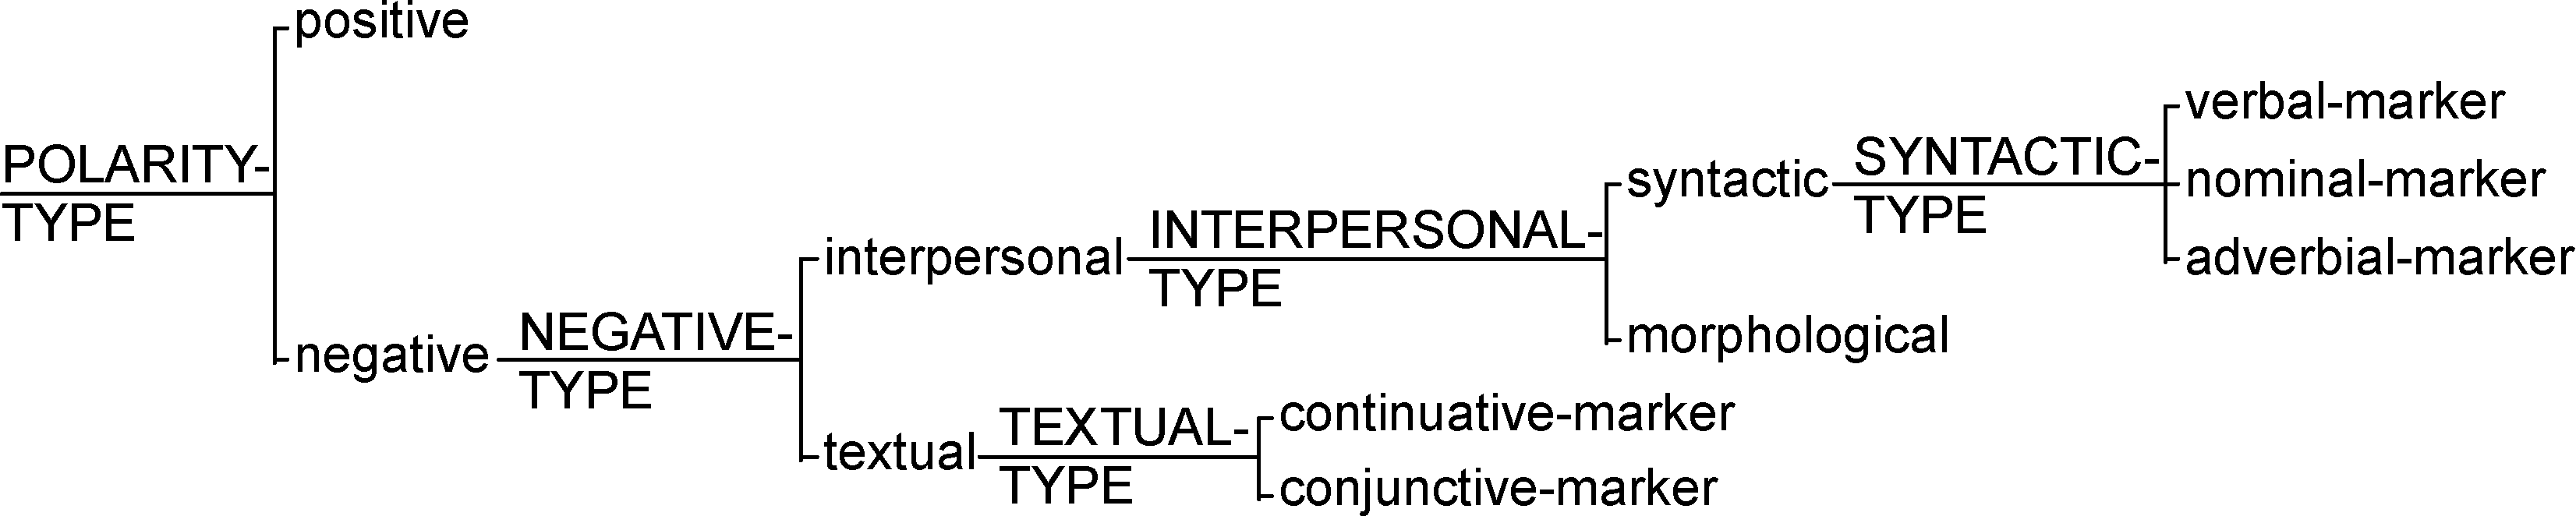
\includegraphics[width=\textwidth]{Figures/SFL-grammar/polarity-system.pdf}
        \caption{Polarity System}
        \label{fig:polarity1}
    \end{figure}

    %The process of creating selection path is sometimes called \textit{system network instantiation}. 
    The selection path is generated by traversal of the feature network from a given feature node towards the root node. If the node has no incoming edge then the result of traversal is a leaf node and the resulting selection path is complete. For example, if \textit{verbal-marker} feature is selected in the system network depicted in Figure \ref{fig:polarity1} the traversal of the corresponding feature network toward root feature yields the selection path \textit{negative -- interpersonal -- syntactic -- verbal-marker}. This path is also complete with respect to the network because there are no systems younger than the SYNTACTIC-TYPE system.

    When the system networks define more than one feature in the precondition it leads to split paths. This means that there is more than one feature that needs to or can be preselected. If the edge is a continuous line (depicted  in Figure \ref{fig:feature-network-example1}) the both variants are part of the same selection path. In case the edge is a dashed line (depicted  in Figure \ref{fig:feature-network-example2}) the paths are considered alternative and a further decision making mechanism must be employed to reduce the disjunction to a single variant. In the current work no such mechanism is employed and the parse result is presented with both alternatives. In most cases the entry condition is constituted of a single feature, when there are multiple ones, usually they are conjuncted and only in a small minority of cases entry condition is a disjunction of features.

    \begin{algorithm}[!ht]
        \Input {\feature, \snet}
        \Begin {
            add \feature to empty selection path \;
            \For{\systemm \KwTo traversal path to the root of \snet}
            {
                get entry condition features of \systemm \;
                add entry condition features to the selection path \;
            }
            \Return{selection path}
        }
        \caption{Naive backwards induction of a selection path}
        \label{alg:backward-induction-naive}
    \end{algorithm}

    The pseudo code for creating a selection path as described above is outlined in Algorithm \ref{alg:backward-induction-naive}. Given a system network and a random non-root feature belonging to the network, it traverses the systems, one by one, towards the root and collects the entry conditions of each system into a selection path.

\section{On realisation rules}
\label{sec:realisation-reules}
    The previous section explains that in the current work system networks are simplified to a taxonomy of features and no realisation rules are considered. This section explains how the pattern graphs are a substitute for the realisation rules and how they relate to each other.

    The \textit{realisation rule} of a systemic feature specifies how that feature is realised as a syntagmatic structure down to a text form using operations such as insert or expand constituent, order two constituent, preselect another feature, lexicalise etc. They are the essential ingredients binding the paradigmatic description in a syntagmatic structure. Robin Fawcett recurrently emphasises the role of realisation rules in the composition of system networks. He often stresses ``no system networks without realisation rules''. It is the \textit{instantiation} process that in Halliday's words ``is the relation between a semiotic system and the \textit{observable} events or `acts' of meaning'' \citep[emphasis added]{Halliday2003-systemic-theory}. The realisation rules for a systemic feature are the statement of operations through which that feature contributes to the structural configuration (that is being either generated or recognised) \citep[p.86]{Fawcett2000}.

    % It is not easy however for linguists and grammarians to provide such statements for the systemic features. Doing so means an explicit formalisation of grammar on top of charting the systemic composition and dependencies which is already a challenging task in its own. Not to mention that writing a good grammar is already a very difficult task. The realisation rules most of the time remain in the minds of the interpreters who can recognise a feature when it occurs. Adding the formal specification of the realisation rule requires tools for consistency checking with respect to the rest of the grammar and large corpus query tool to test various rule hypotheses which are not really available yet. 

    %The graph patterns described in this chapter can be a suitable approach to address the problem of missing realisation rules.

    In this work the graph patterns can be considered as bundles of realisation rules and feature selections and therefore an approach to replace the realisation rules. This idea is implicitly covered in Section \ref{sec:pattern-graphs} and here I explicitly describe it through an example. Consider the fragment of the Mood system network from \citet[162]{Halliday2013} depicted in Figure \ref{fig:mood-fragment}. This example aims at three feature selections: major, indicative and declarative. The root feature in the system network is realised through a constituent \textit{clause}, any of the selected fratures is ascribed directly to it, and the selection of any subsequent features impacts the elements below through the associated realisation rules. The pattern graph that captures selection of the major feature is depicted in Figure \ref{fig:mood-fragment-major}. 

    \begin{figure}[!ht]
        \centering
        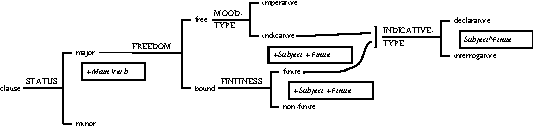
\includegraphics[width=\textwidth]{Figures/Example/mood-fragment.pdf}
        \caption{An adapted fragment of a Mood system from \citep[162]{Halliday2013} }
        \label{fig:mood-fragment}
    \end{figure}

    \begin{figure}[!ht]
        \centering
        \scalebox{0.7}{
        \begin{tikzpicture}[tree-style,level distance=5em,] 
        \node[pattern-node, anchor=center] (c) {class:clause, STATUS:major}
        child {node[pattern-node] (subj1) {element:Main Verb}};
        \end{tikzpicture}
        }
        \caption{A graph pattern for \textit{major} feature selection in Figure \ref{fig:mood-fragment}}
        \label{fig:mood-fragment-major}
    \end{figure}

    Figure \ref{fig:mood-fragment-indicative} depicts the pattern graph corresponding to the selection of indicative feature. Here the clause constituent receives the whole selection path up to the root feature \textit{clause -- major -- free -- indicative} and in addition two more constituents are required: Subject and Finite. Almost the same pattern graph is valid in case of selecting bound feature instead of indicative.

    \begin{figure}[!ht]
        \centering
        \scalebox{0.7}{
        \begin{tikzpicture}[tree-style,level distance=5em,] 
        \node[pattern-node, anchor=center] (c) {class:clause, STATUS:major, FREEDOM:free,\\MOOD-TYPE:indicative }
        child {node[pattern-node] (subj1) {element:Main Verb}}
        child {node[pattern-node] (subj1) {element:Subject}}
        child {node[pattern-node] (subj1) {element:Finite}}
        ;
        \end{tikzpicture}
        }
        \caption{A graph pattern for \textit{indicative} feature selection in Figure \ref{fig:mood-fragment}}
        \label{fig:mood-fragment-indicative}
    \end{figure}
    
    \begin{figure}[!ht]
        \centering
        \scalebox{0.7}{
        \begin{tikzpicture}[tree-style,level distance=5em,] 
        \node[pattern-node, anchor=center] (c) {class:clause, STATUS:major, FREEDOM:free,\\ MOOD-TYPE:indicative, INDICATIVE-TYPE:declarative }
        child {node[pattern-node] (subj1) {element:Main Verb}}
        child {node[pattern-node] (subj1) {element:Subject,\\precede:fnt}}
        child {node[pattern-node] (subj1) {id:fnt,\\element:Finite}}
        ;
        \end{tikzpicture}
        }
        \caption{A graph pattern for \textit{declarative} feature selection in Figure \ref{fig:mood-fragment}}
        \label{fig:mood-fragment-declarative}
    \end{figure}

    In Figure \ref{fig:mood-fragment-declarative} the selection is taken one step further to the declarative feature. The associated realisation rule is ordering the Subject and Finite elements. This is captured via the ``precede:fnt'' where ``fnt'' is the id of the Finite constituent. 

    \begin{figure}[!ht]
        \centering
        \scalebox{0.7}{
        \begin{tikzpicture}[tree-style,level distance=5em,] 
        \node[pattern-node, anchor=center] (c) {MOOD-TYPE:indicative, INDICATIVE-TYPE:declarative }
        child {node[pattern-node] (subj1) {element:Subject,\\precede:fnt}}
        child {node[pattern-node] (subj1) {id:fnt,\\element:Finite}}
        ;
        \end{tikzpicture}
        }
        \caption{A graph pattern for the selection if \textit{indicative} and \textit{declarative} features in Figure \ref{fig:mood-fragment}}
        \label{fig:mood-fragment-declarative-indicative-isolated}
    \end{figure}

    The pattern does not need to refer to the complete selection path but can be limited to the context of a few related features. For example, Figure \ref{fig:mood-fragment-declarative-indicative-isolated} represents selection of the indicative and declarative features in isolation. In this case the class of the parent constituent (that in the above cases is the clause) is no longer specified because the restricted selection path and thus the root of the network is not reached. Also none of the preselected features \textit{major} and \textit{free} are specified either.  

    One limitation, however, of the graph patterns is dealing with conflation phenomena. For example, the cases of the Main Verb conflated with Finite elements have to be accounted by with pattern graphs where one constituent has two functions instead of pattern graphs with two separate constituents each with the corresponding function. This limitation can be addressed in the future by manipulating the definition of the feature structure matcher described in Section \ref{sec:graph-matching}.

\section{Discussion}
    This chapter described from a computer science perspective the SFL concepts introduced in Chapter \ref{ch:sfg} and prepares the ground for the following chapters that address the implementation details of the Parsimonious Vole parser.  

    A central theme covered here are the graphs and graph patterns. They play the key role in identifying grammatical features in dependency and constituency structures. They are also an excellent candidate for expressing \textit{systemic realizations} which have not been considered in the current work as being associated with the systemic features.  

    %In Section \ref{sec:realisation-reules} I mentioned that 
    Authoring realisation rules is a difficult task and requires proper tool support. The same is the case for graph patterns and even more so when they need to be related to systemic networks or network parts. The system network authoring tool, such as the one available in UAM Corpus Tool \citep{ODonnell2008a}, should provide also a graph pattern editor allowing association of graph patterns to systemic features. Unfortunately building such an editor is out of the scope of the current work and is among the priorities in the future developments. Also employing a mature specialised technology for manipulating large amounts of graph data as available in the Semantic Web suite of tools is another direction for the future described in the Section \ref{sec:future-work}.

    In the next chapter I describe the parsing pipeline and how each step is implemented starting from the Stanford dependency graph all the way down to a rich constituency systemic functional parse structure.

    %copied
    %Robin Fawcett recurrently emphasises the role of realization rules in the composition of system networks. He often stresses ``no system networks without realization rules''. They are important because they formally express ways in which a feature is identified or realised. It is the \textit{instantiation} process that in Halliday's words ``is the relation between a semiotic system and the \textit{observable} events or `acts' of meaning'' \citep[emphasis added]{Halliday2003-systemic-theory}. The realisation rules for a systemic feature are the statement of operations through which that feature contributes to the structural configuration (that is being either generated or recognised) \citep[p.86]{Fawcett2000}.
    
    %It is not easy however for linguists and grammarians to provide such statements for the systemic features. Doing so means an explicit formalisation of grammar on top of charting the systemic composition and dependencies which is already a challenging task in its own. The realisation rules most of the time remain in the minds of the interpreters who can recognise a feature when it occurs. Adding the formal specification of the realisation rule requires tools for consistency checking with respect to the rest of the grammar and large corpus query tool to test various rule hypotheses. 
    
    %Moreover the expression of rules is proposed in terms of atomic operations such as lexify, preselect, insert, order, etc. Which may not always be fully transparent to the grammarian. Expressing realization rules as operations contextualised in fragments of parse structure is a promising way to ease the grammar authoring process. They could then be used directly by the parser to recognise such structures making the corpus annotation and grammar construction an in-parallel evolving process.
    
    %The data structures and operations with them described in this chapter can be a suitable approach to address the problem of missing realisation rules from the system networks.
    %To do so however requires creation of a system network authoring tool (such as the one available in UAM Corpus Tool \citep{ODonnell2008a}) which besides systemic network editor should contain also a graph pattern editor allowing association of graph patterns to systemic features. 
    
    %In current parser the pattern graphs are represented as compositions of Python dictionaries and lists such as the one below.
    %%* The Patterns are written as python data structures thus not very user friendly, an editor would be much more helpful
    %\begin{Verbatim}[fontsize=\relsize{-2}]
    %{
    %    NODES: {  
    %        "cl": [
    %            {C_TYPE: 'clause', 
    %             VOICE: ACTIVE},
    %            {CONFIGURATION: ['two-role-action', ['Ag', 'Ra', 'Cre']], }],
    %        'pred': [
    %            {C_TYPE: [PREDICATOR, PREDICATOR_FINITE], }, 
    %            {VERB_TYPE: "main", PROCESS_TYPE: 'two-role-action'} ],
    %        'subj': [
    %            {C_TYPE: SUBJECT, }, 
    %            {PARTICIPANT_ROLE: 'Ag'}],
    %        'compl1': [
    %            {C_TYPE: [COMPLEMENT, COMPLEMENT_DATIVE], },
    %            {PARTICIPANT_ROLE: 'Ra'}],
    %        'compl2': [
    %            {C_TYPE: [COMPLEMENT, COMPLEMENT_ADJUNCT, ], },
    %            {PARTICIPANT_ROLE: 'Cre'}],
    %    },
    %    EDGES: [
    %    ['cl', 'pred', None], 
    %    ['cl', 'subj', None], 
    %    ['cl', 'compl1', None], 
    %    ['cl', 'compl2', None],]
    %}
    %\end{Verbatim}
    %
    %This Python dictionary contains two top keys: NODES defined as  with node identifiers each associated with a set of systemic features and EDGES defined as a list with three tuples of source, target and eventually a dictionary of features. The nodes contain a list of two dictionaries. The first dictionary enlists the features that the backbone structure should already carry, and against which the pattern matching is performed. The second dictionary contains the set of features that the node shall receive in case of a successful match of the entire pattern. 
    
    %Writing such structures is cumbersome and requires in depth knowledge of the parser and employed system networks therefore the need for an editor is even higher. 
    %Unfortunately building such an editor is out of the scope of the current work and is among the priorities in the future developments just as switching to better technology for working with graphs such as Semantic Web suite of tools. This and other future work are described in the Section \ref{sec:future-work}.
    %
    %In the next chapter I describe the parsing pipeline and how each step is implemented starting from Stanford dependency graph all the way down to a rich constituency systemic functional parse structure.